% ==============================================================================
% BÀI BÁO KHOA HỌC M-CDSS (CHUẨN TRIPOD-AI & PROBAST)
% File gốc (Master Document): Biên dịch bằng pdflatex hoặc xelatex + bibtex
% Cấu trúc đa file rõ ràng giúp dễ dàng theo dõi và chỉnh sửa từng phân mục
% ==============================================================================
\documentclass[11pt,a4paper]{article}

% Nạp gói Template Học thuật tùy chỉnh của dự án M-CDSS
\usepackage{templates/mcdss_article}

% Số liệu sinh tự động từ results/registry.json (scripts/export_latex_tables.py)
% AUTO-GENERATED by scripts/export_latex_tables.py from results/registry.json. Do not edit.
\newcommand{\aucLRTab}{0.945}
\newcommand{\aucsdLRTab}{0.000}
\newcommand{\eceLRTab}{0.078}
\newcommand{\deltaLRTab}{+0.013}
\newcommand{\deltaciLRTab}{[-0.005; 0.033]}
\newcommand{\pLRTab}{0.456}
\newcommand{\aucCatBoost}{0.925}
\newcommand{\aucsdCatBoost}{0.003}
\newcommand{\eceCatBoost}{0.061}
\newcommand{\deltaCatBoost}{+0.033}
\newcommand{\deltaciCatBoost}{[0.014; 0.053]}
\newcommand{\pCatBoost}{0.010}
\newcommand{\aucFTT}{0.929}
\newcommand{\aucsdFTT}{0.019}
\newcommand{\eceFTT}{0.092}
\newcommand{\deltaFTT}{+0.010}
\newcommand{\deltaciFTT}{[-0.008; 0.027]}
\newcommand{\pFTT}{0.516}
\newcommand{\aucTfidf}{0.917}
\newcommand{\aucsdTfidf}{0.000}
\newcommand{\eceTfidf}{0.094}
\newcommand{\deltaTfidf}{+0.041}
\newcommand{\deltaciTfidf}{[0.019; 0.065]}
\newcommand{\pTfidf}{0.009}
\newcommand{\aucBertFrozen}{0.899}
\newcommand{\aucsdBertFrozen}{0.027}
\newcommand{\eceBertFrozen}{0.116}
\newcommand{\deltaBertFrozen}{+0.054}
\newcommand{\deltaciBertFrozen}{[0.029; 0.080]}
\newcommand{\pBertFrozen}{0.009}
\newcommand{\aucBertFT}{0.975}
\newcommand{\aucsdBertFT}{0.004}
\newcommand{\eceBertFT}{0.072}
\newcommand{\deltaBertFT}{-0.020}
\newcommand{\deltaciBertFT}{[-0.033; -0.008]}
\newcommand{\pBertFT}{0.012}
\newcommand{\aucConcat}{0.929}
\newcommand{\aucsdConcat}{0.021}
\newcommand{\eceConcat}{0.116}
\newcommand{\deltaConcat}{+0.066}
\newcommand{\deltaciConcat}{[0.048; 0.086]}
\newcommand{\pConcat}{0.009}
\newcommand{\aucXattn}{0.956}
\newcommand{\aucsdXattn}{0.008}
\newcommand{\eceXattn}{0.081}
\newcommand{\aucXattnFT}{0.961}
\newcommand{\aucsdXattnFT}{0.015}
\newcommand{\eceXattnFT}{0.106}
\newcommand{\deltaXattnFT}{+0.000}
\newcommand{\deltaciXattnFT}{[-0.010; 0.010]}
\newcommand{\pXattnFT}{0.930}
\newcommand{\aucEnsemble}{0.978}
\newcommand{\aucsdEnsemble}{0.003}
\newcommand{\eceEnsemble}{0.116}
\newcommand{\deltaEnsemble}{-0.024}
\newcommand{\deltaciEnsemble}{[-0.035; -0.013]}
\newcommand{\pEnsemble}{0.009}
\newcommand{\rqtwoTfidfFull}{0.917}
\newcommand{\rqtwoBertFTFull}{0.974}
\newcommand{\rqtwoBertFrozenFull}{0.895}
\newcommand{\rqtwoXattnFull}{0.954}
\newcommand{\rqtwoTfidfNumMasked}{0.541}
\newcommand{\rqtwoBertFTNumMasked}{0.679}
\newcommand{\rqtwoBertFrozenNumMasked}{0.655}
\newcommand{\rqtwoXattnNumMasked}{0.920}
\newcommand{\rqtwoTfidfNoVitals}{0.885}
\newcommand{\rqtwoBertFTNoVitals}{0.905}
\newcommand{\rqtwoBertFrozenNoVitals}{0.923}
\newcommand{\rqtwoXattnNoVitals}{0.965}
\newcommand{\rqtwoTfidfNarrative}{0.826}
\newcommand{\rqtwoBertFTNarrative}{0.776}
\newcommand{\rqtwoBertFrozenNarrative}{0.777}
\newcommand{\rqtwoXattnNarrative}{0.917}
\newcommand{\eceUncal}{0.079}
\newcommand{\eceTemp}{0.077}
\newcommand{\deploySeed}{101}
\newcommand{\testN}{302}
\newcommand{\cvLRTab}{0.909}
\newcommand{\cvsdLRTab}{0.021}
\newcommand{\cvminLRTab}{0.883}
\newcommand{\cvCatBoost}{0.892}
\newcommand{\cvsdCatBoost}{0.036}
\newcommand{\cvminCatBoost}{0.842}
\newcommand{\cvTfidf}{0.904}
\newcommand{\cvsdTfidf}{0.084}
\newcommand{\cvminTfidf}{0.759}
\newcommand{\cvBertFrozen}{0.833}
\newcommand{\cvsdBertFrozen}{0.064}
\newcommand{\cvminBertFrozen}{0.772}
\newcommand{\cvBertFT}{0.894}
\newcommand{\cvsdBertFT}{0.148}
\newcommand{\cvminBertFT}{0.633}
\newcommand{\cvXattn}{0.949}
\newcommand{\cvsdXattn}{0.016}
\newcommand{\cvminXattn}{0.933}
\newcommand{\cvEnsemble}{0.931}
\newcommand{\cvsdEnsemble}{0.066}
\newcommand{\cvminEnsemble}{0.816}
\newcommand{\tmpBertFrozen}{0.879}
\newcommand{\tmpCatBoost}{0.936}
\newcommand{\tmpTfidf}{0.904}
\newcommand{\tmpXattn}{0.879}
\newcommand{\testSourcePatients}{62}
\newcommand{\allSourcePatients}{478}
\newcommand{\ragCases}{50}
\newcommand{\ragClaims}{200}
\newcommand{\ragGrounded}{199}
\newcommand{\ragSpanMatch}{1.00}
\newcommand{\ragProbes}{50/50}
\newcommand{\ragNotesSource}{data/processed\_rebuilt\_strict/test.parquet}
\newcommand{\latPfiftyMultimodal}{782}
\newcommand{\latPninetyfiveMultimodal}{943}
\newcommand{\latStatusMultimodal}{200}
\newcommand{\latPfiftyBaseline}{203}
\newcommand{\latPninetyfiveBaseline}{332}
\newcommand{\latStatusBaseline}{200}
\newcommand{\latPfiftyExplain}{19}
\newcommand{\latPninetyfiveExplain}{28}
\newcommand{\latStatusExplain}{200}
\newcommand{\latMode}{in\_process\_asgi\_testclient}
\newcommand{\latDevice}{Windows 11 -- AMD64 -- CPU (20 logical cores)}

\IfFileExists{generated/rq3_macros.tex}{% AUTO-GENERATED by scripts/export_latex_tables.py from results/registry.json. Do not edit.
\newcommand{\rqthreeBestDelta}{+0.060}
\newcommand{\rqthreeBestRho}{0.25}
\newcommand{\rqthreeBestSigma}{1}
\newcommand{\rqthreeBaseDelta}{-0.005}
\newcommand{\rqthreePositive}{9/15}
}{}

\begin{document}

% ------------------------------------------------------------------------------
% KHỐI TIÊU ĐỀ & THÔNG TIN TÁC GIẢ
% ------------------------------------------------------------------------------
\mcdsstitle
    {Dung Hợp Đa Phương Thức Dữ Liệu Bảng và Ghi Chú Lâm Sàng cho Chẩn Đoán Phân Biệt Hô Hấp -- Tim Mạch: Đánh Giá Có Kiểm Soát Rò Rỉ, Dư Thừa Phương Thức và Nguyên Mẫu M-CDSS Có Hiệu Chuẩn và Giải Trình Kiểm Chứng Được}
    {Nguyễn Nho Dương\textsuperscript{1}, Lê Tuấn Cảnh\textsuperscript{2}, Nguyễn Văn Cường\textsuperscript{3}}
    {\textsuperscript{1}Trưởng nhóm Học máy \& Mô hình hóa Đa phương thức (Lead ML / Multimodal Modeling) \\
     \textsuperscript{2}Kỹ sư Dữ liệu Y sinh \& Bảo mật Quyền riêng tư (Biomedical Data Engineering \& Privacy) \\
     \textsuperscript{3}Kỹ sư Toàn phần AI, Hệ thống Đa tác tử \& Kiến trúc Phần mềm (Full-Stack AI \& Agent Architecture)}
    {Electronic Health Records (EHR), Multimodal Fusion, Cross-Attention, Shortcut Learning, Data Leakage, Calibration, Retrieval-Augmented Explanation, Decision Curve Analysis, TRIPOD+AI, PROBAST+AI.}

% ------------------------------------------------------------------------------
% PHÂN MỤC 00: TÓM TẮT CÓ CẤU TRÚC (STRUCTURED ABSTRACT)
% ------------------------------------------------------------------------------
% ==============================================================================
% Phân mục 00: Tóm tắt có cấu trúc (TRIPOD+AI) – THÀNH VIÊN 1. Số liệu từ generated/macros.tex.
% ==============================================================================
\begin{clinicalbox}{TÓM TẮT (STRUCTURED ABSTRACT -- TRIPOD+AI)}
\textbf{Bối cảnh:} Các mô hình chẩn đoán dựa trên AI và hồ sơ sức khỏe điện tử (EHR) thường được báo cáo với nguy cơ sai lệch cao; lợi ích của việc dung hợp dữ liệu bảng với ghi chú lâm sàng hiếm khi được so sánh công bằng với các phương án đơn giản. \\[0.4em]
\textbf{Mục tiêu:} Đánh giá có kiểm soát rò rỉ một mô hình dung hợp chú ý chéo (FT-Transformer + Bio\_ClinicalBERT) cho chẩn đoán phân biệt hen, COPD, suy tim và viêm phổi, tìm hiểu nguồn gốc tín hiệu văn bản, và xây dựng nguyên mẫu hỗ trợ quyết định (M-CDSS) có hiệu chuẩn và giải trình kiểm chứng được. \\[0.4em]
\textbf{Phương pháp:} Đoàn hệ bán tổng hợp 2.000 bản ghi (Synthea + MTSamples) sinh từ \allSourcePatients{} bệnh nhân gốc, chia theo nhóm bệnh nhân và nhóm ghi chú nguồn (train/val/test 1.425/273/\testN; tập test gồm \testSourcePatients{} bệnh nhân gốc), kèm kiểm toán rò rỉ ở mức nội dung ghi chú. Kế hoạch phân tích được đăng ký trước: mười mô hình, năm seed, temperature scaling trên validation, CI bootstrap và hiệu chỉnh Holm; phân rã tín hiệu văn bản (che số, bỏ sinh hiệu, chỉ tự sự); mô phỏng bổ trợ có kiểm soát; DCA cho suy tim; độ bền khi thiếu dữ liệu; temporal split; và 5-fold grouped CV (post-hoc). \\[0.4em]
\textbf{Kết quả:} Trên tập test strict, Bio\_ClinicalBERT fine-tune đạt macro AUROC \aucBertFT{} $\pm$ \aucsdBertFT{} và ensemble CatBoost + BERT \aucEnsemble{}; cross-attention đạt \aucXattn{} $\pm$ \aucsdXattn{}, thấp hơn có ý nghĩa so với hai mô hình này ($\Delta=\deltaBertFT$ và $\deltaEnsemble$, $p_{\text{Holm}}\le\pBertFT$) và không khác Logistic Regression chỉ dùng dữ liệu bảng (\aucLRTab). Trong grouped CV, cross-attention ổn định nhất (\cvXattn{} $\pm$ \cvsdXattn{} so với \cvBertFT{} $\pm$ \cvsdBertFT{} của BERT-FT). Khi che mọi con số trong ghi chú, AUROC của BERT-FT giảm từ \rqtwoBertFTFull{} xuống \rqtwoBertFTNumMasked{}: tín hiệu văn bản chủ yếu đến từ sinh hiệu và tuổi được chép lại trong ghi chú. Trong mô phỏng, dung hợp có lợi khi văn bản mang tín hiệu riêng hoặc dữ liệu bảng nhiễu ($\Delta$ lớn nhất \rqthreeBestDelta). Temperature scaling giảm ECE từ \eceUncal{} xuống \eceTemp{}, chưa đạt mục tiêu $<0.05$. Lớp giải trình neo \ragGrounded/\ragClaims{} claim vào đúng vị trí ký tự trong ghi chú và từ chối \ragProbes{} chuỗi ngoài ghi chú. \\[0.4em]
\textbf{Kết luận:} Trên benchmark bán tổng hợp này, chưa có bằng chứng dung hợp chú ý chéo vượt trội; hai ``phương thức'' chồng lấp thông tin và số bệnh nhân gốc quá nhỏ khiến thứ hạng mô hình không bền. Đóng góp chính là quy trình đánh giá có kiểm toán rò rỉ, phân tích cơ chế tín hiệu văn bản và một nguyên mẫu phần mềm tái lập được; cần dữ liệu thật và ngoại kiểm trước mọi ứng dụng lâm sàng.
\end{clinicalbox}


% ------------------------------------------------------------------------------
% PHÂN MỤC 01: MỞ ĐẦU & KHOẢNG TRỐNG NGHIÊN CỨU
% ------------------------------------------------------------------------------
% ==============================================================================
% Phân mục 01: Mở đầu (Introduction) – THÀNH VIÊN 1, Backlog 10 Nhiệm vụ 1.1
% ==============================================================================
\section{Mở Đầu (Introduction)}
\label{sec:introduction}

Phân biệt sớm các nguyên nhân khó thở cấp có biểu hiện chồng lấp -- hen phế quản, bệnh phổi tắc nghẽn mạn tính (COPD), suy tim và viêm phổi mắc phải cộng đồng -- quyết định hướng xử trí ban đầu: thuốc giãn phế quản và corticosteroid, lợi tiểu, hay kháng sinh. Hồ sơ sức khỏe điện tử (EHR) chứa hai loại thông tin bổ sung cho nhau về lý thuyết: dữ liệu có cấu trúc (sinh hiệu, xét nghiệm, nhân khẩu học) và ghi chú lâm sàng tự do (bệnh sử, triệu chứng, đáp ứng điều trị).

Tổng quan hệ thống của Hunik và cộng sự \cite{hunik2024diagnostic} về các mô hình chẩn đoán dựa trên AI và EHR trong chăm sóc ban đầu sàng lọc 10.657 bản ghi và chọn 15 nghiên cứu; theo đánh giá PROBAST \cite{collins2021protocol}, không nghiên cứu nào có nguy cơ sai lệch thấp, chủ yếu do mô tả phương pháp chưa đầy đủ, và các tác giả kết luận chưa mô hình nào sẵn sàng triển khai. Các hướng dẫn mới TRIPOD+AI \cite{collins2024tripod} và PROBAST+AI \cite{probastai2024bmj} nhấn mạnh báo cáo minh bạch, hiệu chuẩn xác suất và kiểm soát rò rỉ dữ liệu. Song song, y văn học máy cho thấy mô hình có thể đạt hiệu năng cao nhờ ``lối tắt'' (\emph{shortcut learning}) \cite{geirhos2020shortcut} hoặc rò rỉ dữ liệu \cite{kapoor2023leakage}, và các khảo sát về học máy đa phương thức trong y khoa \cite{huang2020multimodal,kline2022multimodal} ghi nhận lợi ích của dung hợp thường được báo cáo mà thiếu so sánh với các phương án đơn giản.

Nghiên cứu này xuất phát từ mục tiêu xây dựng một hệ thống hỗ trợ quyết định lâm sàng đa phương thức (M-CDSS) dung hợp FT-Transformer \cite{gorishniy2021revisiting} cho dữ liệu bảng và Bio\_ClinicalBERT \cite{alsentzer2019publicly} cho ghi chú bằng cơ chế chú ý chéo, kèm hiệu chuẩn xác suất \cite{guo2017calibration} và giải trình có trích dẫn kiểm chứng được. Trong quá trình kiểm toán, chúng tôi phát hiện ghi chú của đoàn hệ bán tổng hợp (Synthea \cite{walonoski2018synthea} + MTSamples \cite{mtsamples2012}) chứa lại chính các giá trị sinh hiệu. Vì vậy, thay vì chỉ báo cáo một con số hiệu năng, chúng tôi đặt ra năm câu hỏi nghiên cứu (đăng ký trước, Mục~\ref{sec:methodology}): RQ1 -- so sánh công bằng giữa dung hợp và đơn phương thức; RQ2 -- nguồn gốc tín hiệu văn bản; RQ3 -- điều kiện để dung hợp có ích; RQ4 -- hiệu chuẩn, lợi ích ròng và độ bền khi thiếu dữ liệu; RQ5 -- chất lượng truy xuất và neo bằng chứng.

\paragraph{Đóng góp.}
\begin{itemize}[leftmargin=1.8em, itemsep=0.2em]
  \item \textbf{Quy trình dữ liệu có kiểm toán rò rỉ ở mức nội dung}: chia theo nhóm bệnh nhân và nhóm ghi chú nguồn, khóa thời gian, khử định danh, và kiểm tra tự động tên chẩn đoán chưa che cũng như ghi chú nguồn bị dùng lại mang thông tin nhãn. Kiểm tra này đã phát hiện và loại bỏ một bản dữ liệu trung gian tái đưa rò rỉ vào (Mục~\ref{sec:clinical_cohort}).
  \item \textbf{So sánh công bằng, đăng ký trước}: mười mô hình, năm seed, cùng chế độ backbone cho mô hình văn bản và mô hình dung hợp, CI bootstrap và hiệu chỉnh Holm. Trên tập test strict, dung hợp chú ý chéo \emph{không} vượt mô hình văn bản fine-tune và ensemble đơn giản; trong grouped CV post-hoc, nó lại là mô hình ổn định nhất -- cho thấy thứ hạng mô hình không bền trên đoàn hệ ít bệnh nhân gốc (Mục~\ref{sec:empirical_results}).
  \item \textbf{Phân rã tín hiệu văn bản và mô phỏng bổ trợ có kiểm soát}: chỉ ra rằng lợi thế của mô hình văn bản đến từ các con số trong ghi chú, và xác định điều kiện mà kiến trúc dung hợp khai thác được thông tin bổ trợ thật sự.
  \item \textbf{Nguyên mẫu phần mềm mã nguồn mở có thể tái lập}: dịch vụ suy luận trả xác suất đã hiệu chuẩn, giải trình truy xuất phác đồ với vị trí ký tự kiểm chứng được, giao diện cho bác sĩ, đóng gói Docker, và mọi số liệu trong bài sinh tự động từ một registry kết quả duy nhất.
\end{itemize}

Phần còn lại của bài trình bày đoàn hệ (Mục~\ref{sec:clinical_cohort}), phương pháp (Mục~\ref{sec:methodology}), kiến trúc phần mềm và lớp giải trình (Mục~\ref{sec:software_architecture}--\ref{sec:frontend_dca_ux}), kết quả (Mục~\ref{sec:empirical_results}) và thảo luận (Mục~\ref{sec:discussion_ethics}).


% ------------------------------------------------------------------------------
% PHÂN MỤC 02: ĐOÀN HỆ LÂM SÀNG & QUY TRÌNH DỮ LIỆU (PHỐI HỢP THÀNH VIÊN 2)
% ------------------------------------------------------------------------------
% ==============================================================================
% Phân mục 02: Đoàn hệ Lâm sàng & Quy trình Dữ liệu (Clinical Cohort & Data Pipeline)
% Tác giả phụ trách: Thành viên 2 (Data Engineer & Privacy) - Backlog 10 Nhiệm vụ 2.1
% ==============================================================================
\section{Đoàn Hệ Lâm Sàng và Quy Trình Quản Trị Dữ Liệu (Clinical Cohort \& Data Pipeline)}
\label{sec:clinical_cohort}

\subsection{Thiết Kế Đoàn Hệ và Bản Chất Tạo Dữ Liệu Bán Tổng Hợp (Cohort Genesis \& Simulation Transparency)}
Nhằm khắc phục triệt để các khiếm khuyết phương pháp luận được chỉ ra trong tổng quan hệ thống của Hunik và cộng sự \cite{hunik2024diagnostic} (trong đó đa số nghiên cứu tiền nhiệm gặp nguy cơ sai lệch cao do rò rỉ thông tin hoặc mất đồng bộ thời gian), nghiên cứu này thiết lập đoàn hệ hồi cứu chuẩn hóa gồm $N_{\text{total}} = 2.000$ hồ sơ bệnh án điện tử đa phương thức. 

Để đảm bảo tính trung thực khoa học theo khuyến nghị của TRIPOD+AI \cite{collins2024tripod} và PROBAST+AI \cite{probastai2024bmj}, quy trình kiến tạo đoàn hệ được mô tả minh bạch qua bốn thành phần cốt lõi:
\begin{enumerate}[leftmargin=1.8em, itemsep=0.2em]
    \item \textbf{Dữ liệu dạng bảng từ Synthea EHR:} Vector đặc trưng sinh lý học số hóa ($\bm{x}_{\text{tab}} \in \mathbb{R}^{13}$) được trích xuất từ bộ sinh bệnh nhân tổng hợp \textbf{Synthea} \cite{walonoski2018synthea}, bao gồm $2$ biến nhân khẩu học (Tuổi, Giới tính), $6$ chỉ số sinh hiệu đo đạc lúc tiếp nhận (Huyết áp tâm thu SBP, Huyết áp tâm trương DBP, Nhịp tim HR, Nhịp thở RR, Thân nhiệt Temp, Độ bão hòa oxy máu $\text{SpO}_2$), $2$ chỉ số xét nghiệm phản ứng viêm pha cấp (Bạch cầu WBC, Nồng độ CRP) và $3$ tiền sử bệnh nền/yếu tố nguy cơ (Hút thuốc lá, Tăng huyết áp, Đái tháo đường).
    \item \textbf{Văn bản ghi chú lâm sàng từ MTSamples:} Các phân đoạn văn bản bệnh sử tự do (lý do vào viện, bệnh sử diễn tiến, khám thực thể nghe phổi) được chọn lọc từ kho ghi chú y khoa mở \textbf{MTSamples} \cite{mtsamples2012}, phản ánh ngữ cảnh mô tả lâm sàng phong phú của bác sĩ.
    \item \textbf{Chèn khối sinh hiệu vào văn bản (Cội nguồn phát hiện then chốt RQ2):} Trong quá trình ghép nối bán tổng hợp, một bản mẫu (template) hành chính tiếp nhận được áp dụng, trong đó các chỉ số sinh hiệu đo đạc tại phòng khám ban đầu (ví dụ: \texttt{"BP: 128/82 mmHg, HR: 92 bpm, SpO2: 92\%"}) được chèn trực tiếp vào phần mở đầu của ghi chú tự sự. Sự trùng lặp thông tin này phản ánh đúng thực tế thói quen sao chép kết quả đo vào bệnh án tại phòng khám, nhưng đồng thời tạo ra hiện tượng \textit{dư thừa phương thức (modality redundancy)}. Như được chứng minh trong phần thực nghiệm (RQ2), hiện tượng này chính là nguyên nhân khiến bộ mã hóa văn bản Bio\_ClinicalBERT có thể đạt hiệu năng cao chỉ bằng cách đọc lại các con số sinh hiệu thay vì trích xuất tín hiệu ngữ nghĩa thực sự từ lời văn.
    \item \textbf{Cài cắm thông tin định danh giả lập (Simulated PHI Injection):} Nhằm phục vụ kiểm thử nghiêm ngặt năng lực khử định danh (De-identification) trước khi ứng dụng vào hệ thống thực tế, các trường thông tin nhận dạng cá nhân giả lập đã được tạo lập có chủ đích trong tiêu đề bệnh án: số Căn cước công dân/CMND (12 chữ số), mã số thẻ Bảo hiểm Y tế Việt Nam (tiền tố \texttt{DN4...}), số điện thoại di động, họ tên bệnh nhân, tên bác sĩ kèm học hàm/học vị (\texttt{PGS.TS.}, \texttt{BS.CKII.}) và tên bệnh viện viết HOA toàn bộ (\texttt{BỆNH VIỆN BẠCH MAI}).
\end{enumerate}

Đoàn hệ bao phủ 4 hội chứng tim mạch -- hô hấp gây khó thở phổ biến nhất tại tuyến y tế cơ sở: Hen phế quản (\texttt{ASTHMA}, nhãn 0), Bệnh phổi tắc nghẽn mạn tính (\texttt{COPD}, nhãn 1), Suy tim sung huyết (\texttt{HEART\_FAILURE}, nhãn 2) và Viêm phổi mắc phải cộng đồng (\texttt{PNEUMONIA}, nhãn 3). Đoàn hệ cân bằng hoàn hảo ở mức tổng thể với 500 ca cho mỗi nhóm bệnh lý.

% ==============================================================================
% Hình: Sơ đồ dòng đối tượng theo chuẩn TRIPOD-AI (Flow Diagram of Study Participants)
% M-CDSS Phase 3 / Backlog 10 - Nhiệm vụ 2.1 (Thành viên 2)
% ==============================================================================
\begin{figure}[htbp]
\centering
\resizebox{0.92\textwidth}{!}{%
\begin{tikzpicture}[
    node distance=1.1cm and 1.4cm,
    font=\footnotesize\sffamily,
    >=Stealth
]

    % --- KHỐI NGUỒN DỮ LIỆU ---
    \node[mcdssBox, text width=5.2cm, fill=blue!5] (src_synthea) {
        \textbf{Synthea EHR Simulation}\\
        $N_1 = 2.450$ hồ sơ bệnh nhân tổng hợp\\
        \scriptsize (Dữ liệu bảng: nhân khẩu, sinh hiệu, lab)
    };
    
    \node[mcdssBox, text width=5.2cm, fill=teal!5, right=1.2cm of src_synthea] (src_mtsamples) {
        \textbf{MTSamples Repository}\\
        $N_2 = 4.999$ ghi chú lâm sàng thực tế\\
        \scriptsize (Văn bản tự do: bệnh sử, khám thực thể)
    };

    % --- KHỐI LOẠI TRỪ & LỌC ---
    \node[mcdssBox, text width=4.6cm, draw=mcdssDanger, fill=red!4, below right=0.9cm and -1.8cm of src_synthea] (filter_box) {
        \textbf{Tiêu chí Loại trừ \& Lọc chất lượng}\\
        \scriptsize
        $\bullet$ Bệnh ngoài 4 nhóm mục tiêu ($n = 450$)\\
        $\bullet$ Ghi chú chuyên khoa không khớp ($n = 3.999$)\\
        $\bullet$ Ngoại lai sinh lý vượt ngưỡng can thiệp\\
        $\bullet$ Cấm xét nghiệm tiêu chuẩn vàng: $FEV_1/FVC$, siêu âm tim $LVEF$, cấy đờm vi sinh\\
        $\bullet$ Che từ khóa nhãn (\texttt{[REDACTED\_DIAGNOSIS]})\\
        $\bullet$ Thêm PHI giả lập để kiểm thử de-ID
    };

    % --- KHỐI ĐOÀN HỆ CHUẨN HÓA ---
    \node[mcdssService, text width=7.2cm, fill=mcdssBgLight, below=2.6cm of filter_box] (canonical_cohort) {
        \textbf{Đoàn Hệ Lâm Sàng Chuẩn Hóa M-CDSS ($N = 2.000$)}\\
        \normalfont\scriptsize Cân bằng 4 nhóm bệnh ($25\%$ mỗi nhóm, $n = 500$ ca/bệnh):\\
        Hen phế quản ($500$), COPD ($500$), Suy tim ($500$), Viêm phổi ($500$)
    };

    % --- KHỐI PHÂN CHIA STRICT SPLIT ---
    \node[mcdssBox, text width=3.8cm, fill=green!6, below left=1.2cm and 0.4cm of canonical_cohort] (split_train) {
        \textbf{Tập Huấn Luyện (Train)}\\
        $N_{\text{train}} = 1.425$ ($71,25\%$)\\
        \scriptsize
        Hen: $358$ | COPD: $358$\\
        Suy tim: $340$ | Viêm phổi: $369$\\
        \textit{Khớp tham số mô hình \& MICE}
    };

    \node[mcdssBox, text width=3.8cm, fill=orange!6, below=1.2cm of canonical_cohort] (split_val) {
        \textbf{Tập Hiệu Chuẩn (Val)}\\
        $N_{\text{val}} = 273$ ($13,65\%$)\\
        \scriptsize
        Hen: $71$ | COPD: $71$\\
        Suy tim: $54$ | Viêm phổi: $77$\\
        \textit{Early stopping \& Temperature $T$}
    };

    \node[mcdssBox, text width=3.8cm, fill=purple!6, below right=1.2cm and 0.4cm of canonical_cohort] (split_test) {
        \textbf{Tập Kiểm Thử (Test)}\\
        $N_{\text{test}} = 302$ ($15,10\%$)\\
        \scriptsize
        Hen: $71$ | COPD: $71$\\
        Suy tim: $106$ | Viêm phổi: $54$\\
        \textit{Đánh giá độc lập: AUROC, DCA}
    };

    % --- ĐƯỜNG KẾT NỐI ---
    \coordinate (merge_pt) at ($(src_synthea.south)!0.5!(src_mtsamples.south)$);
    \draw[mcdssArrow] (src_synthea.south) |- (merge_pt) -- (filter_box.north);
    \draw[mcdssArrow] (src_mtsamples.south) |- (merge_pt);
    
    \draw[mcdssArrow] (filter_box.south) -- (canonical_cohort.north);

    \draw[mcdssArrow] (canonical_cohort.south) -| (split_train.north);
    \draw[mcdssArrow] (canonical_cohort.south) -- (split_val.north);
    \draw[mcdssArrow] (canonical_cohort.south) -| (split_test.north);

    % --- KHUNG BAO CHỨNG NHẬN KHÔNG RÒ RỈ ---
    \begin{scope}[on background layer]
        \node[mcdssGroup, fill=gray!3, fit=(split_train) (split_val) (split_test), 
              label={[font=\scriptsize\bfseries\color{mcdssPrimary}]below:Stratified Group Split theo \texttt{patient\_id} \& \texttt{source\_note\_group} (Kiểm toán 0\% rò rỉ: $\mathcal{P}_{\text{train}} \cap \mathcal{P}_{\text{val}} \cap \mathcal{P}_{\text{test}} = \emptyset$)}] (split_group) {};
    \end{scope}

\end{tikzpicture}%
}
\caption{Sơ đồ dòng thiết kế đoàn hệ và phân chia tập dữ liệu M-CDSS theo chuẩn TRIPOD-AI.}
\label{fig:tripod_flow}
\end{figure}


\subsection{Đặc Điểm Lâm Sàng Ban Đầu của Đoàn Hệ (Baseline Characteristics)}
Bảng~\ref{tab:cohort_characteristics} mô tả chi tiết các thông số nhân khẩu học, sinh hiệu và xét nghiệm lâm sàng trên toàn bộ đoàn hệ ($N = 2.000$), phân tách theo các tập phân chia (Train/Val/Test) và phân tách đặc trưng bệnh học theo từng nhóm chẩn đoán mục tiêu. Theo khuyến cáo của chuẩn TRIPOD+AI \cite{collins2024tripod}, các biến số liên tục có phân bố lệch được báo cáo dưới dạng Trung vị kèm Khoảng tứ phân hồi cứu (Median [IQR]), cùng tỷ lệ khuyết thiếu thực tế.

% AUTO-GENERATED by scripts/export_cohort_table.py. Do not edit.
\begin{table}[htbp]\centering\scriptsize
\caption{Đặc điểm đoàn hệ theo split và theo nhóm chẩn đoán (n (\%) hoặc trung vị [IQR]; giá trị sau gán MICE, tỷ lệ thiếu tính từ biến chỉ báo trước gán). Lưu ý tập test có phân bố khác train: toàn bộ ca suy tim trong test là nam và không có người đang hút thuốc.}
\label{tab:cohort_characteristics}
\begin{tabular}{@{}lcccc|cccc@{}}\toprule
Biến & \textbf{Toàn bộ} & \textbf{Train} & \textbf{Val} & \textbf{Test} & \textbf{Hen} & \textbf{COPD} & \textbf{Suy tim} & \textbf{Viêm phổi} \\
 & ($n=2000$) & ($n=1425$) & ($n=273$) & ($n=302$) & ($n=500$) & ($n=500$) & ($n=500$) & ($n=500$) \\ \midrule
Nam & 1088 (54.4\%) & 787 (55.2\%) & 95 (34.8\%) & 206 (68.2\%) & 194 (38.8\%) & 261 (52.2\%) & 335 (67.0\%) & 298 (59.6\%) \\
Đang hút thuốc & 2 (0.1\%) & 2 (0.1\%) & 0 (0.0\%) & 0 (0.0\%) & 0 (0.0\%) & 2 (0.4\%) & 0 (0.0\%) & 0 (0.0\%) \\
Từng hút thuốc & 741 (37.0\%) & 473 (33.2\%) & 126 (46.2\%) & 142 (47.0\%) & 123 (24.6\%) & 146 (29.2\%) & 194 (38.8\%) & 278 (55.6\%) \\
Tăng huyết áp & 644 (32.2\%) & 434 (30.5\%) & 72 (26.4\%) & 138 (45.7\%) & 84 (16.8\%) & 146 (29.2\%) & 303 (60.6\%) & 111 (22.2\%) \\
Đái tháo đường & 823 (41.1\%) & 558 (39.2\%) & 136 (49.8\%) & 129 (42.7\%) & 58 (11.6\%) & 164 (32.8\%) & 376 (75.2\%) & 225 (45.0\%) \\
Tuổi (năm) & 61 [29--97] & 65 [30--97] & 61 [23--97] & 61 [32--61] & 25 [18--41] & 35 [19--53] & 71 [61--96] & 100 [97--100] \\
HA tâm thu (mmHg) & 118 [111--125] & 118 [111--125] & 113 [106--119] & 118 [113--125] & 121 [114--126] & 119 [112--128] & 118 [111--124] & 114 [106--119] \\
HA tâm trương (mmHg) & 80 [76--84] & 80 [76--84] & 80 [78--84] & 81 [77--85] & 80 [76--84] & 79 [75--83] & 80 [77--84] & 81 [77--85] \\
Nhịp tim (/phút) & 79 [69--88] & 81 [71--89] & 83 [72--88] & 68 [65--74] & 76 [68--87] & 79 [68--89] & 78 [67--83] & 85 [73--89] \\
Nhịp thở (/phút) & 14 [13--15] & 14 [13--15] & 14 [13--15] & 15 [14--16] & 14 [13--15] & 14 [13--15] & 15 [14--16] & 15 [14--16] \\
Thân nhiệt ($^\circ$C) & 37.4 [37.0--37.8] & 37.5 [37.1--37.8] & 37.4 [37.0--37.8] & 37.3 [36.7--37.7] & 37.4 [37.0--37.7] & 37.5 [37.0--37.8] & 37.3 [36.9--37.7] & 37.6 [37.1--37.8] \\
SpO$_2$ (\%) & 92.3 [83.7--95.6] & 92.4 [84.3--95.7] & 92.7 [88.6--95.6] & 91.0 [69.0--95.2] & 94.2 [91.4--96.5] & 93.8 [90.6--96.7] & 77.1 [69.0--79.8] & 94.1 [91.6--96.8] \\
Bạch cầu ($10^9$/L) & 7.1 [6.0--8.5] & 7.1 [5.8--8.4] & 7.5 [6.3--9.4] & 7.2 [6.7--7.8] & 7.5 [6.5--8.7] & 7.2 [5.6--8.2] & 6.8 [5.8--7.2] & 7.2 [6.6--9.4] \\
CRP (mg/L) & 13.9 [5.1--19.7] & 13.9 [4.8--19.6] & 13.9 [8.5--21.5] & 13.9 [5.2--19.4] & 13.9 [3.7--20.5] & 13.9 [5.9--19.1] & 13.9 [5.4--19.1] & 13.9 [5.9--20.2] \\
Thiếu WBC trước gán MICE & 410 (20.5\%) & 287 (20.1\%) & 54 (19.8\%) & 69 (22.8\%) & 104 (20.8\%) & 104 (20.8\%) & 106 (21.2\%) & 96 (19.2\%) \\
Thiếu CRP trước gán MICE & 447 (22.4\%) & 327 (22.9\%) & 59 (21.6\%) & 61 (20.2\%) & 101 (20.2\%) & 117 (23.4\%) & 116 (23.2\%) & 113 (22.6\%) \\
Ghi chú dạng MTSamples & 305 (15.2\%) & 208 (14.6\%) & 46 (16.8\%) & 51 (16.9\%) & 83 (16.6\%) & 76 (15.2\%) & 87 (17.4\%) & 59 (11.8\%) \\
\bottomrule\end{tabular}\end{table}


\paragraph{Bất thường của dữ liệu tổng hợp (quan trọng cho diễn giải kết quả).} Bảng~\ref{tab:cohort_characteristics} cho thấy đoàn hệ có những đặc điểm không hợp lý về mặt lâm sàng: tuổi trung vị của nhóm COPD chỉ khoảng 35 trong khi nhóm viêm phổi tập trung quanh 100 tuổi, và SpO$_2$ trung vị của nhóm suy tim thấp bất thường (khoảng 77\%). Vì vậy tuổi và SpO$_2$ gần như tự phân tách các lớp (Logistic Regression chỉ với tuổi đạt macro AUROC khoảng 0.81 trên tập test). Quan trọng hơn, 2.000 bản ghi được sinh từ chỉ \textbf{478 bệnh nhân Synthea gốc} (lớp viêm phổi: 8 bệnh nhân gốc; hen và suy tim: 57; COPD: 402), mỗi bệnh nhân gốc đóng góp nhiều lần khám. Việc chia theo nhóm nguồn ngăn rò rỉ giữa các split nhưng làm tập test strict chỉ còn 	estSourcePatients{} bệnh nhân gốc: \textbf{toàn bộ 106 bản ghi suy tim và 54 bản ghi viêm phổi trong test mỗi lớp đến từ một bệnh nhân gốc} (vì vậy mọi ca suy tim trong test là nam và không có người đang hút thuốc). Hệ quả: hiệu năng theo lớp và DCA cho suy tim thực chất mô tả hành vi trên một bệnh nhân tổng hợp, và khoảng tin cậy bootstrap theo bản ghi đánh giá thấp độ bất định (Mục~\ref{sec:methodology}). Mọi kết quả hiệu năng trong bài cần được hiểu trong bối cảnh này: chúng mô tả hành vi của các mô hình trên một benchmark tổng hợp có tín hiệu nhân khẩu học mạnh, không phải độ khó của bài toán lâm sàng thực.

\subsection{Quy Trình Khử Định Danh Bảo Vệ Quyền Riêng Tư (HIPAA Safe-Harbor De-Identification)}
Để đảm bảo an toàn tuyệt đối cho người bệnh và tuân thủ các quy định quốc tế (HIPAA Safe Harbor \cite{hhs2012hipaa}, GDPR Điều 9) cũng như Nghị định 13/2023/NĐ-CP của Chính phủ Việt Nam về bảo vệ dữ liệu cá nhân, module \texttt{ClinicalDeidentifier} thực thi pipeline làm sạch 18 nhóm thông tin định danh cá nhân (PHI) qua kiến trúc lai ghép:
\begin{enumerate}[leftmargin=1.8em, itemsep=0.2em]
    \item \textbf{Động cơ Biểu thức chính quy nâng cao (Advanced Regex Engine):} Được nâng cấp toàn diện trong Backlog 08 để loại bỏ các dạng thức PHI đặc thù của Việt Nam:
    \begin{itemize}[leftmargin=1.5em, itemsep=0.1em]
        \item Mã thẻ BHYT Việt Nam theo cấu trúc mới: \texttt{\textbackslash b[A-Z]\{2\}\textbackslash d\{1,2\}\textbackslash d\{10,13\}\textbackslash b} (loại bỏ hoàn toàn các mã dạng \texttt{DN418667188111}).
        \item Tên bác sĩ kèm học hàm, học vị y khoa Việt Nam: biểu thức \texttt{(?:GS|PGS|TS|ThS|BS|BSCK|CKI\{1,2\})\textbackslash.?(?:\textbackslash s*[A-Z]+\textbackslash.)*\textbackslash s+[A-ZĐ][\textbackslash wÀ-ỹ]+...} nhận diện chính xác các tiền tố như \texttt{PGS.TS. Lê Hoàng Nam}, \texttt{BS.CKII. Nguyễn Văn Bình}.
        \item Tên cơ sở y tế viết HOA toàn bộ: \texttt{\textbackslash bBỆNH VIỆN(?:\textbackslash s+[A-ZĐÀ-Ỹ0-9]+)+\textbackslash b} che phủ triệt để các tiêu đề như \texttt{BỆNH VIỆN BẠCH MAI}, \texttt{BỆNH VIỆN CHỢ RẪY}.
        \item Số Căn cước công dân/CMND (9--12 chữ số), số điện thoại di động Việt Nam (đầu số \texttt{03, 05, 07, 08, 09} hoặc mã quốc tế \texttt{+84}), địa chỉ email và các mốc ngày tháng (\texttt{DD/MM/YYYY}, \texttt{YYYY-MM-DD}).
    \end{itemize}
    \item \textbf{Động cơ Nhận diện thực thể tên riêng y sinh (Biomedical NER Engine):} Sử dụng mô hình NLP chuyên biệt để phát hiện tên cá nhân (\texttt{PERSON}), cơ sở khám chữa bệnh (\texttt{FACILITY}), và địa danh nhỏ hơn cấp tỉnh/thành phố (\texttt{GPE}).
    \item \textbf{Thay thế bằng Token ngữ cảnh chuẩn hóa (Surrogate Masking):} Các thực thể nhạy cảm bị phát hiện được thay thế bằng token đại diện đồng nhất: \texttt{[REDACTED\_NAME]}, \texttt{[REDACTED\_DATE]}, \texttt{[REDACTED\_PHONE]}, \texttt{[REDACTED\_HOSPITAL]}, \texttt{[REDACTED\_ID]}. Phương pháp này bảo toàn cấu trúc ngữ pháp và tính liền mạch ngữ nghĩa, giúp mô hình ngôn ngữ Bio\_ClinicalBERT tiếp thu ngữ cảnh mà không thể tái định danh đối tượng.
    \item \textbf{Bảo toàn tuyệt đối chỉ số sinh hiệu (Negative Testing):} Kiểm thử tự động trên toàn bộ các chuỗi sinh hiệu viết tắt (\texttt{BP}, \texttt{HR}, \texttt{SpO2}, \texttt{WBC}, \texttt{CRP}, \texttt{Temp}) xác nhận tỷ lệ che nhầm là $0\%$, bảo toàn toàn vẹn dữ liệu lâm sàng đầu vào.
\end{enumerate}

\subsection{Cơ Chế Khóa Chuỗi Thời Gian và Loại Trừ Tiêu Chuẩn Vàng (Temporal Locking \& Anti-Leakage)}
Hiện tượng rò rỉ thông tin tương lai (\textit{Look-ahead Bias / Target Leakage}) là sai sót phổ biến hàng đầu trong các mô hình AI chẩn đoán, xảy ra khi thông tin cận lâm sàng phát sinh sau khi chẩn đoán đã hoàn tất bị đưa nhầm vào tập huấn luyện \cite{kapoor2023leakage,hunik2024diagnostic}. Nghiên cứu thực thi hai hàng rào kỹ thuật nghiêm ngặt:
\begin{enumerate}[leftmargin=1.8em, itemsep=0.2em]
    \item \textbf{Khóa chuỗi thời gian quan sát (\textit{Chronological Time-Locking}):} Module \texttt{TemporalAligner} thiết lập mốc thời gian nghiêm ngặt: gọi $t_{\text{diag}}$ là thời điểm bác sĩ xác lập kết luận chẩn đoán mã ICD-10 trong hệ thống EHR. Mọi dữ liệu biến số đầu vào $X_j(t)$ bắt buộc phải thỏa mãn:
    \begin{equation}
        t(X_j) < t_{\text{diag}}
    \end{equation}
    Bất kỳ chỉ số xét nghiệm hoặc ghi chú điều trị nào phát sinh tại mốc $t \ge t_{\text{diag}}$ đều bị loại bỏ tự động khỏi ma trận đầu vào của mô hình.
    \item \textbf{Danh mục cấm xét nghiệm tiêu chuẩn vàng (\textit{Gold-Standard Blacklist}):} Để khắc phục triệt để nghịch lý chẩn đoán bị JMIR phê phán (ví dụ: dùng đo phế dung khí chẩn đoán Hen/COPD hoặc dùng siêu âm tim chẩn đoán suy tim), hệ thống cấm tuyệt đối đưa các tiêu chuẩn vàng vào dữ liệu đầu vào:
    \begin{itemize}[leftmargin=1.5em, itemsep=0.1em]
        \item Cấm chỉ số Hô hấp ký/Phế dung ký ($FEV_1, FVC, FEV_1/FVC$ sau nghiệm pháp giãn phế quản) vốn là tiêu chuẩn vàng định nghĩa COPD theo GOLD 2024 \cite{gold2024copd}.
        \item Cấm chỉ số Phân suất tống máu thất trái LVEF trên Siêu âm tim Doppler màu (tiêu chuẩn vàng phân loại suy tim HFrEF/HFpEF theo ESC 2023 \cite{mcdonagh2023esc}).
        \item Cấm kết quả cấy đờm vi sinh định danh vi khuẩn và kháng sinh đồ (tiêu chuẩn vàng viêm phổi).
        \item Loại bỏ và che phủ mọi từ khóa chẩn đoán trực tiếp trong văn bản bằng token \texttt{[REDACTED\_DIAGNOSIS]}.
    \end{itemize}
\end{enumerate}

\subsection{Phân Chia Tập Dữ Liệu Nghiêm Ngặt Theo Bệnh Nhân (Patient-Level Group Splitting)}
Khi một bệnh nhân có nhiều đợt khám hoặc nhiều bản ghi tiến triển trong hệ thống, việc phân chia ngẫu nhiên thông thường (\textit{Random Splitting}) sẽ làm phân tán các bản ghi của cùng một bệnh nhân sang cả tập Train và tập Test. Hiện tượng này tạo ra rò rỉ định danh bệnh nhân (\textit{Identity Confounding}), khiến mô hình học thuộc đặc điểm cá nhân thay vì học quy luật bệnh học tổng quát.

Để ngăn chặn triệt để nguy cơ này, nghiên cứu áp dụng kỹ thuật \textbf{Stratified Group Splitting} (\texttt{StratifiedGroupKFold}) với tỷ lệ phân chia 70\% Huấn luyện ($N = 1.425$), 15\% Kiểm định ($N = 273$) và 15\% Kiểm thử độc lập ($N = 302$). Phân chia được nhóm hóa đồng thời theo cả mã định danh bệnh nhân (\texttt{patient\_id}) và nguồn gốc văn bản gốc (\texttt{source\_note\_group}), đảm bảo tính tách biệt tuyệt đối về mặt toán học:
\begin{equation}
    \mathcal{P}_{\text{train}} \cap \mathcal{P}_{\text{val}} = \emptyset, \quad \mathcal{P}_{\text{train}} \cap \mathcal{P}_{\text{test}} = \emptyset, \quad \mathcal{P}_{\text{val}} \cap \mathcal{P}_{\text{test}} = \emptyset
\end{equation}
Toàn bộ quá trình phân chia đã được kiểm toán tự động qua tập lệnh \texttt{scripts/audit\_data\_leakage.py} (báo cáo lưu tại \texttt{data/rebuilt\_strict\_split_audit.json}), xác nhận $0$ trường hợp rò rỉ bệnh nhân giữa các tập dữ liệu.

\subsection{Nội Suy Đa Biến MICE Kèm Biến Chỉ Báo Khuyết Thiếu (MICE Imputation with Indicators)}
Trong thực hành lâm sàng ngoại trú ban đầu, dữ liệu cận lâm sàng thường xuyên bị thiếu khuyết có chủ đích (\textit{Missing Not At Random --- MNAR}): bác sĩ chỉ chỉ định xét nghiệm công thức máu WBC hoặc định lượng CRP khi bệnh nhân có biểu hiện sốt, ho đờm đục hoặc nghi ngờ nhiễm khuẩn cấp tính. Do đó, việc xóa bỏ dòng chứa dữ liệu khuyết (\textit{Complete Case Analysis}) sẽ làm mất đi 30\%--40\% đối tượng nghiên cứu và gây méo mó nghiêm trọng phân bố bệnh nhân.

Nghiên cứu sử dụng thuật toán \textbf{Nội suy Đa biến bằng Phương trình Chuỗi liên kết (MICE)} \cite{vanbuuren2011mice} qua module \texttt{ClinicalImputer} (\texttt{sklearn.impute.IterativeImputer}), tuân thủ nghiêm ngặt kỷ luật học máy y tế:
\begin{enumerate}[leftmargin=1.8em, itemsep=0.2em]
    \item \textbf{Kỷ luật Fit-Transform chặt chẽ:} Bộ nội suy MICE chỉ được khớp tham số hồi quy (\texttt{fit}) duy nhất trên tập Huấn luyện (\texttt{train.parquet}), sau đó áp dụng phép biến đổi suy luận (\texttt{transform}) sang tập Validation và Test. Nghiêm cấm tuyệt đối việc fit bộ nội suy trên toàn bộ dữ liệu gộp.
    \item \textbf{Bổ sung Biến chỉ báo khuyết thiếu (Missingness Indicators):} Đối với mỗi biến số có tỷ lệ khuyết thiếu (WBC khuyết 14.4\%, CRP khuyết 19.1\% trên toàn bộ đoàn hệ), hệ thống tự động sinh thêm biến nhị phân chỉ thị $I_{\text{missing}} \in \{0, 1\}$ (\texttt{wbc\_missing}, \texttt{crp\_missing}). Cơ chế này cho phép mô hình học được giá trị chẩn đoán tiềm ẩn từ chính hành vi ``không chỉ định xét nghiệm'' của bác sĩ điều trị.
\end{enumerate}


% ------------------------------------------------------------------------------
% PHÂN MỤC 03: PHƯƠNG PHÁP LUẬN DUNG HỢP & HIỆU CHUẨN (PHỐI HỢP THÀNH VIÊN 1)
% ------------------------------------------------------------------------------
% ==============================================================================
% Phân mục 03: Phương pháp – mô hình, thiết kế thực nghiệm và phân tích thống kê
% [THÀNH VIÊN 1 – BACKLOG 10 NHIỆM VỤ 1.1]. Kế hoạch phân tích đăng ký trước:
% docs/11_ANALYSIS_PLAN.md (phụ lục A, hash đóng băng tại results/preregistration/).
% ==============================================================================
\section{Phương Pháp (Methods)}
\label{sec:methodology}

\subsection{Câu hỏi nghiên cứu}
Nghiên cứu trả lời năm câu hỏi đã đăng ký trước khi chạy thực nghiệm:
\textbf{RQ1} -- dưới so sánh công bằng (cùng split, cùng chế độ huấn luyện backbone, nhiều seed, khoảng tin cậy), dung hợp chú ý chéo có vượt mô hình đơn phương thức tốt nhất và các cách dung hợp đơn giản không;
\textbf{RQ2} -- tín hiệu dự báo của nhánh văn bản đến từ đâu;
\textbf{RQ3} -- trong điều kiện nào thì dung hợp thực sự có ích (mô phỏng có kiểm soát);
\textbf{RQ4} -- mô hình có hiệu chuẩn, có lợi ích ròng (DCA) và bền vững khi thiếu một phương thức không;
\textbf{RQ5} -- lời giải trình có neo vào bằng chứng và truy xuất đúng phác đồ không (Mục~\ref{sec:multi_agent_rag}).

\subsection{Bộ mã hóa từng phương thức}
\textbf{Nhánh bảng (FT-Transformer \cite{gorishniy2021revisiting}).} Chín biến số liên tục (chuẩn hóa theo trung bình/độ lệch chuẩn của tập huấn luyện) và bốn biến danh mục được ánh xạ thành token $\bm{t}_j\in\mathbb{R}^{d}$, $d=128$:
\begin{equation}
  \bm{t}_j^{(\text{num})}=x_j\,\bm{W}_j+\bm{b}_j,\qquad
  \bm{T}_{\text{tab}}=\mathrm{TransformerEncoder}_{4\times}\big([\bm{t}_{\text{[CLS]}},\bm{t}_1,\dots,\bm{t}_{13}]\big)\in\mathbb{R}^{14\times d}.
\end{equation}
\textbf{Nhánh văn bản (Bio\_ClinicalBERT \cite{alsentzer2019publicly}).} Ghi chú đã khử định danh được tách thành tối đa $L=512$ subword token. Mười một khối encoder đầu luôn đóng băng; trạng thái đầu ra khối 11 được tính một lần và lưu lại. Khối encoder cuối được chạy lại trong mỗi bước huấn luyện ở một trong hai chế độ: \emph{đóng băng} (cho đầu ra trùng khớp tuyệt đối với \texttt{last\_hidden\_state} của mô hình gốc, sai khác tối đa $0{,}0$) hoặc \emph{fine-tune} (khối cuối được cập nhật với tốc độ học $2\times10^{-5}$). Đầu ra được chiếu tuyến tính về $\bm{H}_{\text{text}}\in\mathbb{R}^{L\times d}$. Thiết kế này cho phép so sánh mô hình chỉ văn bản và mô hình dung hợp \emph{dưới cùng một chế độ backbone}, điều mà thực nghiệm Giai đoạn 2 chưa đảm bảo.

\subsection{Đầu dung hợp}
\textbf{Cross-attention có cổng.} Token \texttt{[CLS]} của nhánh bảng làm truy vấn trên các token văn bản không phải padding:
\begin{equation}
  \bm{c}=\mathrm{softmax}\!\Big(\tfrac{(\bm{t}_{\text{[CLS]}}\bm{W}_Q)(\bm{H}_{\text{text}}\bm{W}_K)^\top}{\sqrt{d_k}}+\bm{M}_{\text{pad}}\Big)\bm{H}_{\text{text}}\bm{W}_V,\qquad
  \bm{g}=\sigma\big(\bm{W}_g[\bm{t}_{\text{[CLS]}};\bm{c}]\big),\quad
  \bm{h}=\bm{g}\odot\bm{t}_{\text{[CLS]}}+(1-\bm{g})\odot\bm{c},
\end{equation}
với 4 đầu chú ý; $\bm{z}=\bm{W}_o\,\mathrm{LN}(\bm{h})\in\mathbb{R}^4$.
\textbf{Concat fusion} (đối chứng): $\bm{z}=\bm{W}\,\mathrm{LN}([\bm{t}_{\text{[CLS]}};\overline{\bm{H}}_{\text{text}}])$ với $\overline{\bm{H}}_{\text{text}}$ là trung bình các token hợp lệ.
\textbf{Ensemble xác suất} (đối chứng): trung bình xác suất đã hiệu chuẩn của CatBoost và Bio\_ClinicalBERT fine-tune cùng seed.

\subsection{Huấn luyện và hiệu chuẩn}
Mọi mạng nơ-ron dùng AdamW (tốc độ học đầu phân loại $2\times10^{-4}$, weight decay $10^{-5}$), batch 32, tối đa 12 epoch, dừng sớm khi NLL validation không giảm sau 4 epoch, cắt gradient chuẩn 1,0 và mixed precision. Logistic Regression và TF-IDF + LR chọn hệ số điều chuẩn $C\in\{0{,}25;1;4;16\}$ theo NLL validation; CatBoost dùng siêu tham số cố định trong \texttt{configs/model\_config.yaml}. Với \emph{mọi} mô hình, xác suất được hiệu chuẩn bằng temperature scaling \cite{guo2017calibration}, $\hat p_c=\exp(z_c/T)/\sum_j\exp(z_j/T)$, với $T$ tối ưu theo NLL trên tập validation ($N=273$); với mô hình sklearn, $z=\log\hat p$. Tập kiểm thử chỉ được dùng để báo cáo.

\subsection{Thiết kế thực nghiệm}
\textbf{RQ1.} Mười mô hình (Bảng~\ref{tab:rq1}) huấn luyện với 5 seed (13, 42, 101, 2024, 7); mô hình tất định chạy một lần. Seed đại diện của mỗi mô hình là seed có NLL validation thấp nhất; checkpoint triển khai là cross-attention đóng băng ở seed đại diện. Mô hình triển khai được chọn \emph{trước} khi xem kết quả test vì tương thích với dịch vụ suy luận (BERT đầy đủ, đóng băng).

\textbf{RQ2 -- phân rã tín hiệu văn bản.} Bốn biến thể ghi chú được tạo bằng hàm tất định: \emph{gốc}; \emph{che số} (mọi chữ số $\to$ \texttt{<NUM>}); \emph{bỏ sinh hiệu} (bỏ khối VITALS và mọi câu chứa sinh hiệu/xét nghiệm có giá trị số); \emph{chỉ tự sự} (chỉ lý do khám, bệnh sử, thuốc). TF-IDF + LR, BERT (đóng băng, fine-tune) và cross-attention được huấn luyện lại trên từng biến thể với 3 seed.

\textbf{RQ3 -- mô phỏng bổ trợ có kiểm soát.} Trên biến thể che số, một câu triệu chứng đặc hiệu theo lớp (diễn giải từ tiêu chuẩn chẩn đoán GINA, GOLD, ESC, Bộ Y tế) được chèn vào đầu bệnh sử cho tỷ lệ $\rho\in\{0;0{,}25;0{,}5;0{,}75;1\}$ bệnh nhân; 10\% câu chèn lấy từ lớp sai. Nhiễu Gauss $\sigma\in\{0;0{,}5;1\}\times$SD được cộng vào chín biến số. Đại lượng báo cáo: $\Delta=\text{AUROC}_{\text{fusion}}-\max(\text{AUROC}_{\text{bảng}},\text{AUROC}_{\text{văn bản}})$. Đây là \emph{mô phỏng cơ chế}, tín hiệu do nhóm nghiên cứu thiết kế, không phản ánh hiệu năng lâm sàng.

\textbf{RQ4.} (a) Hiệu chuẩn: không hiệu chuẩn, temperature, vector scaling và isotonic one-vs-rest, đều khớp trên validation. (b) DCA \cite{vickers2006decision,vickers2016netbenefit}: suy tim one-vs-rest, hành động giả định là chỉ định NT-proBNP và siêu âm tim, dải ngưỡng $p_t\in[0{,}05;0{,}30]$; số can thiệp giảm ròng trên 100 bệnh nhân $=(\text{NB}-\text{NB}_{\text{all}})(1-p_t)/p_t\times100$. (c) Thiếu phương thức lúc suy luận: ghi chú rỗng; toàn bộ biến bảng thay bằng trung vị/mode của train; thiếu ngẫu nhiên 10/30/50\% biến số (thay bằng trung vị). (d) Temporal split có tôn trọng nhóm nguồn (70/15/15 theo thời điểm khám sớm nhất của nhóm) -- kiểm tra độ bền nội bộ trên dấu thời gian tổng hợp, không phải ngoại kiểm.

\textbf{Phân tích độ nhạy post-hoc.} Do tập test strict có phân bố nhân khẩu học khác tập huấn luyện (Mục~\ref{sec:clinical_cohort}), chúng tôi bổ sung 5-fold grouped cross-validation trên toàn bộ 2.000 ca (seed 42). Phân tích này được đăng ký bổ sung sau khi thấy phân bố test nhưng trước khi chạy, và được gắn nhãn post-hoc.

\subsection{Phân tích thống kê}
Chỉ số chính là macro AUROC one-vs-rest; chỉ số phụ gồm macro AUPRC, macro-F1 (argmax), Brier đa lớp và ECE (10 bin độ rộng bằng nhau; phụ: 15 bin equal-mass và classwise ECE). Kết quả đa seed được báo cáo dạng trung bình $\pm$ độ lệch chuẩn. Khoảng tin cậy 95\% dùng bootstrap theo bản ghi (mỗi \texttt{patient\_id}; $B=2000$, phân vị) trên seed đại diện. Vì các bản ghi được sinh từ một số ít bệnh nhân Synthea gốc (chỉ 	estSourcePatients{} bệnh nhân gốc trong tập test, trong đó suy tim và viêm phổi mỗi lớp chỉ một bệnh nhân), CI này \emph{đánh giá thấp} độ bất định thực; bootstrap theo cụm bệnh nhân gốc không khả thi vì hai lớp chỉ có một cụm. so sánh cặp dùng \emph{cùng} các mẫu bootstrap cho hai mô hình, $p$ hai phía từ phân phối bootstrap của hiệu số, hiệu chỉnh Holm trên 9 so sánh với mô hình triển khai. Toàn bộ số liệu trong bài được sinh tự động từ \texttt{results/registry.json} bằng \texttt{scripts/export\_latex\_tables.py}.


% ------------------------------------------------------------------------------
% PHÂN MỤC 04 [TRỌNG TÂM NHIỆM VỤ 3.2]: KIẾN TRÚC PHẦN MỀM & GIAO THỨC RESTFUL
% ------------------------------------------------------------------------------
% ==============================================================================
% Phân mục 04 [TRỌNG TÂM NHIỆM VỤ 3.2]: Kiến trúc Phần mềm & Giao thức RESTful
% ==============================================================================
\section{Kiến Trúc Phần Mềm Đa Tầng và Giao Thức Hợp Đồng Dữ Liệu RESTful (Software Architecture)}
\label{sec:software_architecture}

Để chuyển hóa các mô hình học sâu đa phương thức từ môi trường thử nghiệm rời rạc thành một hệ thống hỗ trợ quyết định lâm sàng có khả năng vận hành thực tế tại bàn khám bệnh, M-CDSS được thiết kế theo kiến trúc vi dịch vụ 3 tầng tách biệt (\textit{Decoupled Three-Tier Microservice Architecture}). Toàn bộ kiến trúc được minh họa chi tiết tại Hình~\ref{fig:system_architecture}.

% ==============================================================================
% Hình 1: Sơ đồ Kiến trúc Phần mềm Đa tầng M-CDSS (Vector TikZ)
% ==============================================================================
\begin{figure}[htbp]
\centering
\resizebox{\textwidth}{!}{%
\begin{tikzpicture}[node distance=1.2cm and 1.6cm]

    % --- TẦNG 1: PRESENTATION TIER (NEXT.JS 14 FRONTEND - PORT 3000) ---
    \node[mcdssBox] (ui_form) {
        \textbf{PatientDataForm.tsx}\\
        \scriptsize Nhập 12 sinh hiệu \& bệnh án
    };
    \node[mcdssBox, below=0.7cm of ui_form] (ui_card) {
        \textbf{DiagnosticCard.tsx}\\
        \scriptsize Thanh xác suất hiệu chuẩn ($\text{ECE}<0.05$)
    };
    \node[mcdssBox, below=0.7cm of ui_card] (ui_ev) {
        \textbf{EvidenceViewer \& Drawer}\\
        \scriptsize Highlight $[start, end]$ \& CPGs
    };
    \node[mcdssBox, below=0.7cm of ui_ev] (ui_dca) {
        \textbf{DCACurveChart.tsx}\\
        \scriptsize Đồ thị Net Benefit ($p_t \in [0.05, 0.60]$)
    };

    \begin{scope}[on background layer]
        \node[mcdssGroup, fill=blue!3, fit=(ui_form) (ui_dca), label={[font=\footnotesize\bfseries\sffamily, text=mcdssPrimary]above:Tầng Giao Diện (Next.js 14 :3000)}] (tier_frontend) {};
    \end{scope}

    % --- TẦNG 2: APPLICATION & API GATEWAY TIER (FASTAPI - PORT 8000) ---
    \node[mcdssService, right=2.4cm of ui_form] (api_pred) {
        POST /api/v1/predict/mock\\
        \normalfont\scriptsize Multimodal \& Baseline Inference
    };
    \node[mcdssService, right=2.4cm of ui_card] (api_agent) {
        POST /api/v1/agent/explain\\
        \normalfont\scriptsize Multi-Agent RAG \& Grounding
    };
    \node[mcdssService, right=2.4cm of ui_ev] (api_eval) {
        GET /api/v1/evaluation/benchmark\\
        \normalfont\scriptsize Metrics, DCA Points \& PROBAST
    };
    \node[mcdssService, right=2.4cm of ui_dca] (api_health) {
        GET /health \& Pydantic V2\\
        \normalfont\scriptsize Kiểm soát biên sinh lý \& CORS
    };

    \begin{scope}[on background layer]
        \node[mcdssGroup, fill=teal!3, fit=(api_pred) (api_health), label={[font=\footnotesize\bfseries\sffamily, text=mcdssSecondary]above:Tầng Điều Phối RESTful (FastAPI :8000)}] (tier_api) {};
    \end{scope}

    % --- TẦNG 3: AI CORE & DATA PERSISTENCE TIER ---
    \node[mcdssBox, right=2.4cm of api_pred, text width=3.9cm] (core_fusion) {
        \textbf{Multimodal Fusion Engine}\\
        \scriptsize FT-Transformer + Bio\_ClinicalBERT\\
        Cross-Attention + Temp Scaling ($T$)
    };
    \node[mcdssAgent, right=2.4cm of api_agent, text width=3.9cm] (core_agent) {
        \textbf{Agentic RAG \& Grounder}\\
        \scriptsize LangGraph Orchestrator +\\
        Kiểm chứng vị trí ký tự $\mathcal{O}(N)$
    };
    \node[mcdssBox, right=2.4cm of api_eval, text width=3.9cm] (core_qdrant) {
        \textbf{Qdrant Vector DB (:6333)}\\
        \scriptsize Kho phác đồ GINA, GOLD, ESC\\
        Hybrid Search (Dense + BM25)
    };
    \node[mcdssBox, right=2.4cm of api_health, text width=3.9cm] (core_store) {
        \textbf{Strict Split Benchmarks}\\
        \scriptsize Tập kiểm thử độc lập ($N=302$)\\
        0\% Patient-level Leakage
    };

    \begin{scope}[on background layer]
        \node[mcdssGroup, fill=orange!3, fit=(core_fusion) (core_store), label={[font=\footnotesize\bfseries\sffamily, text=mcdssAccent]above:Tầng Lõi AI \& Lưu Trữ Tri Thức}] (tier_core) {};
    \end{scope}

    % --- KẾT NỐI MŨI TÊN (REST JSON & INTERNAL CALLS) ---
    \draw[mcdssArrow, <->] (ui_form.east) -- node[above, font=\tiny\sffamily] {JSON Payload} (api_pred.west);
    \draw[mcdssArrow, <->] (ui_card.east) -- node[above, font=\tiny\sffamily] {Calibrated $P(y|x)$} (api_pred.west);
    \draw[mcdssArrow, <->] (ui_ev.east) -- node[above, font=\tiny\sffamily] {Spans + CPGs} (api_agent.west);
    \draw[mcdssArrow, <->] (ui_dca.east) -- node[above, font=\tiny\sffamily] {DCA \& PROBAST} (api_eval.west);

    \draw[mcdssArrow] (api_pred.east) -- (core_fusion.west);
    \draw[mcdssArrow] (api_agent.east) -- (core_agent.west);
    \draw[mcdssDashedArrow, <->] (core_agent.south) -- node[right, font=\tiny\sffamily] {Top-$k$ Chunks} (core_qdrant.north);
    \draw[mcdssArrow] (api_eval.east) -- (core_store.west);

\end{tikzpicture}%
}
\caption{Kiến trúc phần mềm 3 tầng đóng gói trong mạng nội bộ Docker (\texttt{mcdss-internal-net}), kết nối giao diện bác sĩ (Next.js 14), cổng điều phối hợp đồng dữ liệu (FastAPI) và lõi suy luận đa phương thức cùng kho vector y văn (Qdrant).}
\label{fig:system_architecture}
\end{figure}



\subsection{Phân tách Trách nhiệm Ba Tầng Dịch vụ}
Kiến trúc hệ thống tuân thủ nguyên lý tách biệt mối quan tâm (\textit{Separation of Concerns}) thông qua ba dịch vụ độc lập giao tiếp qua mạng nội bộ ảo \texttt{mcdss-internal-net}:
\begin{enumerate}[leftmargin=1.8em, itemsep=0.25em]
    \item \textbf{Tầng Giao diện Lâm sàng (\textit{Presentation Tier} --- Next.js 14, Cổng 3000):} Được xây dựng bằng \texttt{React 18} và \texttt{TypeScript} theo kiến trúc \textit{App Router}. Tầng này cung cấp bàn làm việc hội chẩn tương tác cho bác sĩ (\texttt{PatientDataForm}, \texttt{DiagnosticCard}, \texttt{EvidenceViewer}, \texttt{GuidelineDrawer}) và bảng điều khiển thẩm định lâm sàng (\texttt{DCACurveChart}). Để tối ưu hóa dung lượng đóng gói, ứng dụng được biên dịch ở chế độ độc lập (\texttt{output: "standalone"}) qua quy trình Docker đa tầng (\textit{Multi-stage build}).
    \item \textbf{Tầng Điều phối \& Hợp đồng Dữ liệu (\textit{Application \& API Gateway Tier} --- FastAPI, Cổng 8000):} Đóng vai trò cổng giao tiếp RESTful trung tâm vận hành trên máy chủ bất đồng bộ \texttt{Uvicorn}. Tầng này thực thi kiểm định biên sinh lý chặt chẽ bằng \texttt{Pydantic V2} trước khi chuyển luồng dữ liệu tới lõi suy luận đa phương thức hoặc dịch vụ giải trình (\texttt{agent\_chat.py}).
    \item \textbf{Tầng Lõi Suy luận AI \& Cơ sở dữ liệu Vector (\textit{AI Core \& Persistence Tier} --- PyTorch \& Qdrant, Cổng 6333):} Bao gồm mô hình dung hợp \texttt{MultimodalEHRClassifier} đã hiệu chuẩn nhiệt độ và cơ sở dữ liệu vector \texttt{Qdrant} lưu trữ các phân đoạn phác đồ điều trị y khoa chính thống (GINA, GOLD, ESC, Bộ Y tế).
\end{enumerate}

\subsection{Thiết kế Giao thức RESTful và Kiểm định Biên Sinh lý Tự động}
Trong tin học y tế, việc truyền nhầm đơn vị đo lường hoặc nhập các giá trị sinh hiệu phi sinh lý (ví dụ: $\text{SpO}_2 > 100\%$ hoặc nhịp tim âm) có thể khiến mô hình học sâu đưa ra dự đoán sai lệch nguy hiểm. Do đó, mọi yêu cầu HTTP gửi tới tầng Backend đều bắt buộc đi qua lớp kiểm định hợp đồng dữ liệu \texttt{TabularFeatures} (\texttt{src/api/schemas.py}):
\begin{itemize}[leftmargin=1.8em, itemsep=0.2em]
    \item \textbf{Ràng buộc miền giá trị sinh lý (\textit{Physiological Domain Constraints}):} Tuổi bệnh nhân $\in [0, 120]$ năm; Huyết áp tâm thu $\in [40, 300]\text{ mmHg}$; Huyết áp tâm trương $\in [20, 200]\text{ mmHg}$; Nhịp tim $\in [20, 300]\text{ bpm}$; Nhịp thở $\in [4, 80]\text{ lần/phút}$; Thân nhiệt $\in [30.0, 45.0]^\circ\text{C}$; Độ bão hòa oxy máu $\text{SpO}_2 \in [50.0, 100.0]\%$.
    \item \textbf{Ràng buộc toàn vẹn văn bản bệnh án (\textit{Clinical Note Validation}):} Trường \texttt{clinical\_note} bắt buộc có độ dài tối thiểu hợp lệ sau khi cắt bỏ khoảng trắng thừa; mọi yêu cầu vi phạm bị chặn ngay tại tầng cổng với mã trạng thái \texttt{HTTP 422} hoặc \texttt{400}.
    \item \textbf{Định chuẩn Tiên đề Xác suất (\textit{Probability Axiom Enforcement}):} Tại đầu ra, lớp kiểm định \texttt{PredictionResponse} xác nhận vector xác suất dự đoán trên 4 nhóm bệnh thỏa mãn $\sum_{c=1}^{4} \hat{p}_c = 1.0 \pm 10^{-3}$ trước khi trả về cho trình duyệt của bác sĩ.
\end{itemize}

Bảng~\ref{tab:rest_endpoints} tổng hợp toàn bộ hệ thống điểm cuối RESTful API phục vụ luồng hội chẩn và kiểm định lâm sàng.

\begin{table}[htbp]
\centering
\caption{Đặc tả các điểm cuối giao thức RESTful API trọng tâm của hệ thống M-CDSS.}
\label{tab:rest_endpoints}
\footnotesize
\begin{tabularx}{\textwidth}{@{}llX@{}}
\toprule
\textbf{Phương thức \& Đường dẫn} & \textbf{Schema Đầu ra Chính} & \textbf{Chức năng Lâm sàng \& Đảm bảo Kỹ thuật} \\
\midrule
\texttt{GET /health} & \texttt{HealthResponse} & Kiểm tra trạng thái sống (\textit{Liveness/Readiness}) của container API và kết nối nội bộ Docker. \\[0.4em]
\texttt{POST /api/v1/predict/mock} & \texttt{PredictionResponse} & Thực thi suy luận đa phương thức (hoặc đối chứng với 3 mô hình Baseline), trả về phân phối xác suất đã hiệu chuẩn ($\text{ECE} < 0.05$) và trọng số chú ý chéo. \\[0.4em]
\texttt{POST /api/v1/agent/explain} & \texttt{AgentExplainResponse} & Thực thi quy trình giải trình tất định (\texttt{deterministic\_template}), truy xuất lai Qdrant--BM25 và trả về danh sách câu bằng chứng đã xác thực tọa độ ký tự $[\text{start\_char}, \text{end\_char}]$ kèm bản kiểm toán \texttt{ClaimAudit}. \\[0.4em]
\texttt{GET /api/v1/benchmarks/baselines} & \texttt{BaselineBenchmarkList} & Xuất ma trận chỉ số định lượng của 3 mô hình đơn phương thức trên tập kiểm thử độc lập ($N=302$). \\[0.4em]
\texttt{GET /api/v1/benchmarks/ablation} & \texttt{AblationBenchmarkList} & Cung cấp kết quả thực nghiệm cắt bỏ thành phần (\textit{Ablation Study}) chứng minh đóng góp của tầng Cross-Attention và Temperature Scaling. \\[0.4em]
\texttt{GET /api/v1/evaluation/benchmark} & \texttt{EvaluationBenchmark} & Tính toán động tọa độ đường cong quyết định DCA ($p_t \in [0.05, 0.60]$) qua \texttt{dca\_analysis.py} và trả về bảng kiểm 4 miền PROBAST. \\
\bottomrule
\end{tabularx}
\end{table}


% ------------------------------------------------------------------------------
% PHÂN MỤC 05 [TRỌNG TÂM NHIỆM VỤ 3.2]: ĐA TÁC TỬ RAG & NEO BẰNG CHỨNG KÝ TỰ
% ------------------------------------------------------------------------------
% ==============================================================================
% Phân mục 05 [TRỌNG TÂM NHIỆM VỤ 3.2]: Hệ thống Đa tác tử & Neo bằng chứng
% ==============================================================================
\section{Hiện Thực Quy Trình Truy Xuất Phác Đồ và Neo Bằng Chứng Ký Tự (Guideline RAG \& Character-Offset Grounding)}
\label{sec:multi_agent_rag}

Một trong những yêu cầu khắt khe nhất của y học chứng cứ (\textit{Evidence-Based Medicine}) là mọi gợi ý chẩn đoán phân biệt phải truy nguyên được về hai nguồn căn cứ độc lập: (1) triệu chứng cụ thể ghi nhận trên chính bệnh nhân đó, và (2) điều khoản tương ứng trong hướng dẫn thực hành lâm sàng chính thống. Để giảm nguy cơ sinh trích dẫn không có căn cứ từ bệnh án, chúng tôi hiện thực hóa quy trình giải trình lâm sàng tất định kết hợp bộ truy xuất lai Qdrant--BM25 và bộ kiểm chứng tọa độ ký tự, được minh họa tại Hình~\ref{fig:multi_agent_rag_flow}.

% ==============================================================================
% Hình 2: Luồng Hội Chẩn Đa Tác Tử & Truy Xuất Tri Thức Lai (Agentic RAG Flow)
% ==============================================================================
\begin{figure}[htbp]
\centering
\resizebox{\textwidth}{!}{%
\begin{tikzpicture}[node distance=1.1cm and 1.3cm]

    % Input node
    \node[mcdssBox, fill=blue!5, text width=3.1cm] (input) {
        \textbf{Đầu vào Hội chẩn}\\
        \scriptsize Sinh hiệu $\bm{x}_{\text{tab}}$, Bệnh án $T$,\\
        Xác suất $\hat{\bm{p}}$ (Top-1, Top-2)
    };

    % Node 1: Triage & Query Formulation
    \node[mcdssAgent, right=1.2cm of input, text width=3.3cm] (triage) {
        \textbf{1. Tác tử Phân loại}\\
        \scriptsize (\textit{Triage \& Query Node})\\
        Trích xuất hội chứng \& tạo truy vấn y khoa
    };

    % Node 2: Hybrid Retriever
    \node[mcdssService, right=1.2cm of triage, text width=3.5cm] (retriever) {
        \textbf{2. Truy xuất Lai}\\
        \normalfont\scriptsize (\textit{HybridGuidelineRetriever})\\
        0.65 Từ khóa Y khoa + 0.35 Vector Ngữ nghĩa
    };

    % Node 3: Diagnostic Synthesis
    \node[mcdssAgent, below=1.2cm of retriever, text width=3.5cm] (synthesis) {
        \textbf{3. Tác tử Tổng hợp}\\
        \scriptsize (\textit{Clinical Reasoning Node})\\
        Đối chiếu chẩn đoán phân biệt \& trích dẫn CPG
    };

    % Node 4: Evidence Grounder
    \node[mcdssService, left=1.2cm of synthesis, text width=3.3cm, draw=mcdssDanger] (grounder) {
        \textbf{4. Bộ Kiểm Chứng}\\
        \normalfont\scriptsize (\textit{EvidenceGrounder} $\mathcal{O}(N)$)\\
        Đối sánh chuỗi con \& tính tọa độ $[start, end]$
    };

    % Output Verified
    \node[mcdssBox, left=1.2cm of grounder, fill=teal!8, text width=3.1cm] (output) {
        \textbf{Báo cáo Đã Xác thực}\\
        \scriptsize \texttt{hallucination\_free: true}\\
        Highlight câu bệnh án \& điều khoản GINA/GOLD
    };

    % Arrows
    \draw[mcdssArrow] (input) -- (triage);
    \draw[mcdssArrow] (triage) -- node[above, font=\tiny\sffamily] {Query + Disease Filter} (retriever);
    \draw[mcdssArrow] (retriever) -- node[right, font=\tiny\sffamily] {Top-$k$ Phác đồ} (synthesis);
    \draw[mcdssArrow] (synthesis) -- node[above, font=\tiny\sffamily] {Candidate Spans} (grounder);
    \draw[mcdssArrow] (grounder) -- node[above, font=\tiny\sffamily] {100\% Khớp gốc} (output);

    % Anti-hallucination rejection loop
    \draw[mcdssDashedArrow, draw=mcdssDanger] (grounder.south) -- ++(0,-0.55) -| node[pos=0.25, below, font=\tiny\sffamily\bfseries, text=mcdssDanger] {Loại bỏ câu trích dẫn không tồn tại trong văn bản gốc (Anti-Hallucination Gate)} (synthesis.south);

\end{tikzpicture}%
}
\caption{Đồ thị trạng thái hội chẩn đa tác tử (\textit{Multi-Agent Diagnostic StateGraph}). Mọi câu trích dẫn chứng cứ do tác tử sinh ra đều phải đi qua cổng kiểm chứng tất định \texttt{EvidenceGrounder} trước khi hiển thị cho bác sĩ.}
\label{fig:multi_agent_rag_flow}
\end{figure}


\subsection{Kiến trúc Quy trình Giải trình \& Kiểm chứng Hiện thực (\texttt{agent\_chat.py})}
Luồng suy luận giải trình tại điểm cuối \texttt{POST /api/v1/agent/explain} (\texttt{src/api/routes/agent\_chat.py}) vận hành ở chế độ \texttt{reasoning\_mode = "deterministic\_template"} phối hợp với bộ truy xuất phác đồ lai và cổng kiểm chứng tọa độ ký tự qua 4 bước tuần tự:
\begin{enumerate}[leftmargin=1.8em, itemsep=0.2em]
    \item \textbf{Khử định danh \& Xác định cặp giả thuyết:} Tiếp nhận bệnh án gốc, thực thi ẩn danh hóa qua \texttt{ClinicalDeidentifier}, ưu tiên cặp chẩn đoán cạnh tranh cao nhất (Top-1 và Top-2) từ vector xác suất đã hiệu chuẩn (\texttt{calibrated\_probabilities}), đồng thời rà quét các dấu hiệu cờ đỏ (\textit{Red Flags}).
    \item \textbf{Truy xuất Tri thức Lai Qdrant--BM25 (\texttt{HybridGuidelineRetriever} --- \texttt{src/agent/retriever.py}):} Kết hợp tìm kiếm từ khóa thưa \textbf{BM25} trên kho 64 phân mảnh JSON chuẩn hóa (\texttt{data/guidelines/*.json}; lớp hạt giống nội bộ \texttt{STANDARD\_GUIDELINE\_CORPUS} chỉ dùng làm dự phòng khi thư mục JSON rỗng) và truy vấn vector dày đặc qua \textbf{Qdrant} (\texttt{query\_points}, 768 chiều với mô hình \texttt{sentence-transformers/all-mpnet-base-v2} theo \texttt{configs/rag\_config.yaml} hoặc hàm băm tất định $L_2$ khi chạy offline; cảnh báo rõ và hỗ trợ \texttt{strict\_qdrant=True} không nuốt lỗi khi Qdrant lỗi). Hai danh sách xếp hạng được hợp nhất bằng kỹ thuật \textbf{Reciprocal Rank Fusion (RRF)}:
    \begin{equation}
        S_{\text{RRF}}(q, d_k) = \sum_{r \in \{\text{BM25}, \text{Dense}\}} \frac{1}{60 + \text{rank}_r(q, d_k)}
    \end{equation}
    trong đó thành phần BM25 trên tập ứng viên được tính theo công thức chuẩn:
    \begin{equation}
        \text{BM25}(q, d_k) = \sum_{t \in q} \ln\!\left(1 + \frac{N_{\text{doc}} - \text{df}(t) + 0.5}{\text{df}(t) + 0.5}\right) \cdot \frac{\text{tf}(t, d_k) \cdot (k_1 + 1)}{\text{tf}(t, d_k) + k_1 \cdot \left(1 - b + b \cdot \frac{|d_k|}{\text{avgdl}}\right)}, \quad k_1 = 1.2,\; b = 0.75
    \end{equation}
    \begin{itemize}[leftmargin=1.5em, itemsep=0.15em]
        \item \textit{Quy mô kho tri thức phác đồ đã chuẩn hóa:} Hệ thống \texttt{knowledge\_ingest.py} đã mở rộng và xác minh đồng bộ ở chế độ chỉ đọc (\textit{read-only verify} chiều vector \texttt{768}, tập \texttt{chunk\_id}, mã băm SHA-256 của \texttt{text\_content} và 8 trường metadata truy nguyên theo tỷ lệ \texttt{64/64}; \textbf{không} xác nhận chất lượng ngữ nghĩa của các vector băm ngoại tuyến) kho tri thức gồm \textbf{64 đoạn chuẩn hóa} (trên đĩa \texttt{data/guidelines/*.json} $=$ trong RAM BM25 $=$ trong Qdrant sống \texttt{clinical\_guidelines}), phân bổ đều 16 đoạn/bệnh lý từ GINA 2024, GOLD 2024, ESC 2023 và Bộ Y tế Việt Nam 2020; bảo toàn \texttt{evidence\_level = null} cho tài liệu Bộ Y tế Việt Nam 2020.
        \item \textit{Đánh giá mô hình nhúng \& Truy xuất RAG (RQ5 --- Thực nghiệm đo đạc trực tiếp trên Qdrant Docker sống với 60 truy vấn bằng vector băm 768-D ngoại tuyến):} Bộ kiểm định chỉ đọc \texttt{scripts/eval\_rag.py} đánh giá qua Qdrant HTTP thực tế (\texttt{http://127.0.0.1:6333}, \texttt{strict\_qdrant=True}) trên 60 truy vấn lâm sàng gán nhãn kép độc lập quy chiếu toàn bộ vào 64 chunk chuẩn hóa (15 truy vấn/bệnh, hệ số đồng thuận $\kappa_{\text{Cohen}} = 0.9449$). Kết quả so sánh 3 cấu hình được trình bày ở Bảng~\ref{tab:rag_eval}. Cần nhấn mạnh rằng toàn bộ kết quả Recall/MRR/nDCG hiện tại đo trong cấu hình chạy ngoại tuyến thiếu trọng số \texttt{all-mpnet-base-v2}, tức nhánh dense dùng bộ mã hóa băm tất định 768 chiều (\textit{768d\_hashed\_deterministic\_cpu\_fallback}, chưa đại diện cho chất lượng encoder ngữ nghĩa thật đang ở trạng thái chờ): \texttt{dense\_only} đạt $R@1 = 0.7833$ và $R@3 = 0.9167$, trong khi \texttt{hybrid\_rrf} hợp nhất với BM25 đạt $R@1 = 0.9000$, $R@3 = 0.9500$, $R@5 = 1.0000$ và $\text{MRR} = 0.9319$. Chế độ sinh lập luận bằng LLM chưa được triển khai và là hướng phát triển (Mục~\ref{sec:discussion_ethics}).
    \end{itemize}

\begin{table}[htbp]
\centering
\caption{Kết quả thực nghiệm truy xuất phác đồ RAG trên 60 truy vấn gán nhãn kép ($\kappa = 0.9449$, 64 đoạn xác minh đọc-chỉ chiều 768/ID/SHA-256/8 metadata trong Qdrant sống; \textbf{dùng vector băm 768-D ngoại tuyến, chưa dùng encoder ngữ nghĩa \texttt{all-mpnet-base-v2}})}
\label{tab:rag_eval}
\begin{tabularx}{\linewidth}{@{}lrrrrr@{}}
\toprule
\textbf{Cấu hình truy xuất} & \textbf{Recall@1} & \textbf{Recall@3} & \textbf{Recall@5} & \textbf{MRR} & \textbf{nDCG@5} \\
\midrule
\texttt{dense\_only} (768-D hash fallback --- chờ \texttt{mpnet}) & 0.7833 & 0.9167 & 0.9833 & 0.8688 & 0.8729 \\
\texttt{bm25\_only} & 0.9000 & 0.9500 & 1.0000 & 0.9319 & 0.9354 \\
\texttt{hybrid\_rrf} (Qdrant hash + BM25 RRF --- chờ \texttt{mpnet}) & 0.9000 & 0.9500 & 1.0000 & 0.9319 & 0.9354 \\
\bottomrule
\end{tabularx}
\end{table}

\textbf{Kiểm tra bất biến tọa độ và từ chối chuỗi ngoài văn bản trên tập test strict:} \texttt{eval\_rag.py} chạy luồng \texttt{explain\_clinical\_case()} trên \ragCases{} ghi chú lấy từ \texttt{\ragNotesSource} (tập strict $N=\testN$, không dùng ghi chú mẫu). Có \ragGrounded/\ragClaims{} claim ứng viên được neo; mọi đoạn đã neo thỏa bất biến $T[\text{start}:\text{end}] \equiv \text{text}$ (tỷ lệ \ragSpanMatch), và \ragProbes{} đầu dò chuỗi không có trong bệnh án bị từ chối. \textit{Giới hạn:} các chỉ số này chỉ chứng minh tính nhất quán vị trí ký tự và khả năng lọc chuỗi ngoài ghi chú; chúng \textbf{không} đo ảo giác theo nghĩa ngữ nghĩa, xử lý phủ định hay giá trị lâm sàng. Đánh giá ngữ nghĩa thủ công 20 đoạn trích (\texttt{results/grounding\_manual\_audit\_20\_samples.json}) \textbf{chưa được thực hiện} tại thời điểm viết bài; chỉ số \texttt{manual\_semantic\_precision} vì vậy không được báo cáo.
\item \textbf{Tổng hợp Lập luận Theo Mẫu Tất định (\textit{Deterministic Template Reasoning}):} Sinh câu đối chiếu chẩn đoán $H_1$ so với $H_2$, kèm theo thông báo rõ trạng thái xác minh nguồn (\texttt{source\_id}, \texttt{version}, \texttt{section\_locator}, \texttt{source\_verified}) của phác đồ trích dẫn và danh sách các câu ứng viên $\{s_1, s_2, \dots, s_m\}$. Chế độ suy luận bằng LLM (tuỳ chọn trong kế hoạch) \textbf{không được triển khai}; mọi kết quả giải trình trong bài thuộc chế độ tất định \texttt{deterministic\_template}..
    \item \textbf{Cổng Kiểm chứng Tọa độ Ký tự (\texttt{EvidenceGrounder} --- \texttt{src/agent/evidence\_grounder.py}):} Thực thi kiểm duyệt vị trí ký tự đối với toàn bộ câu ứng viên trước khi phản hồi xuống Frontend.
\end{enumerate}

\subsection{Thuật toán Neo Bằng chứng Ký tự $\mathcal{O}(N)$ (Character-Offset Evidence Grounding)}
Để hạn chế giao diện tô sáng các câu trích dẫn không tồn tại nguyên văn trong hồ sơ bệnh án đã khử định danh (\texttt{display\_note}), module \texttt{EvidenceGrounder} thực thi đối sánh chuỗi con tất định 3 tầng (khớp chính xác, không phân biệt hoa/thường, chuẩn hóa khoảng trắng), loại bỏ các đoạn chồng lấn (\texttt{resolve\_overlapping\_spans}), và trả về kiểm toán chi tiết \texttt{ClaimAudit} tách biệt giữa \textit{vị trí span khớp chuỗi} với \textit{nhận định lâm sàng cần bác sĩ kiểm chứng độc lập} (Hình~\ref{fig:evidence_grounding}).

% ==============================================================================
% Hình 3: Cơ chế Neo Bằng Chứng Ký Tự (Character-Offset Evidence Grounding)
% ==============================================================================
\begin{figure}[htbp]
\centering
\resizebox{0.96\textwidth}{!}{%
\begin{tikzpicture}[node distance=0.9cm and 1.2cm]

    % Raw Note Box
    \node[mcdssBox, text width=13.5cm, align=left, fill=mcdssBgLight] (raw_note) {
        \textbf{Văn bản bệnh án gốc ($T$, độ dài $N$ ký tự --- Ví dụ Ca PT-0044):}\\[0.2em]
        \texttt{\footnotesize "... Patient is an \colorbox{yellow!35}{\textbf{18yo female presenting with acute wheezing}} and shortness of breath after exercise. History of childhood asthma, currently using \colorbox{teal!25}{\textbf{albuterol inhaler PRN}} ..."}
    };

    % Candidate Spans
    \node[mcdssAgent, below left=1.0cm and -2.2cm of raw_note, text width=5.8cm, align=left] (cand_valid) {
        \textbf{Trích dẫn ứng viên hợp lệ $s_1$:}\\
        \texttt{\scriptsize "18yo female presenting with acute wheezing"}\\
        $\rightarrow$ Khớp chính xác tại $[start=18, end=60]$
    };

    \node[mcdssBox, below right=1.0cm and -2.2cm of raw_note, text width=5.8cm, align=left, draw=mcdssDanger, fill=red!4] (cand_invalid) {
        \textbf{Trích dẫn ảo giác $s_{\text{hallucinated}}$:}\\
        \texttt{\scriptsize "Spirometry shows FEV1/FVC ratio of 0.58"}\\
        $\rightarrow$ Không tồn tại trong $T$ ($\text{find}(s) = -1$)
    };

    % Verification Engine
    \node[mcdssService, below=2.6cm of raw_note, text width=8.5cm] (verifier) {
        \textbf{Thuật toán Đối sánh Tất định \texttt{EvidenceGrounder.verify\_and\_locate()}}\\
        \normalfont\scriptsize Độ phức tạp $\mathcal{O}(N)$ $\cdot$ Chuẩn hóa khoảng trắng $\cdot$ Bất biến chữ hoa/thường
    };

    % Final UI Output
    \node[mcdssBox, below=0.9cm of verifier, text width=11.0cm, fill=teal!6] (ui_render) {
        \textbf{Payload JSON trả về cho \texttt{EvidenceViewer.tsx}:}\\
        \texttt{\scriptsize \{"start\_char": 18, "end\_char": 60, "verified": true, "clinical\_rationale": "Khởi phát trẻ tuổi + ran rít cấp"\}}
    };

    % Connections
    \draw[mcdssArrow] (raw_note.south) -- (cand_valid.north);
    \draw[mcdssArrow, draw=mcdssDanger] (raw_note.south) -- (cand_invalid.north);
    \draw[mcdssArrow] (cand_valid.south) -- node[left, font=\tiny\sffamily\bfseries, text=mcdssSecondary] {Chấp nhận (Verified)} (verifier.north west);
    \draw[mcdssDashedArrow, draw=mcdssDanger] (cand_invalid.south) -- node[right, font=\tiny\sffamily\bfseries, text=mcdssDanger] {Bác bỏ tức thì (Rejected)} (verifier.north east);
    \draw[mcdssArrow] (verifier.south) -- (ui_render.north);

\end{tikzpicture}%
}
\caption{Cơ chế kiểm chứng vị trí ký tự $\mathcal{O}(N)$ trong \texttt{EvidenceGrounder}: Chỉ những chuỗi con tồn tại nguyên vẹn trong văn bản gốc mới được cấp tọa độ $[start, end]$ để tô sáng trên giao diện bác sĩ; mọi suy diễn ngoài văn bản đều bị chặn hoàn toàn.}
\label{fig:evidence_grounding}
\end{figure}



Nhờ cơ chế đối sánh tất định này, mọi đối tượng \texttt{EvidenceSpan} gửi xuống thành phần \texttt{EvidenceViewer.tsx} đều thỏa mãn bất biến cắt chuỗi trên văn bản đã khử định danh $T = \texttt{display\_note}$:
\begin{equation}
    0 \le \text{start\_char} < \text{end\_char} \le |T| \quad \text{và} \quad T[\text{start\_char}:\text{end\_char}] \equiv \text{text}
\end{equation}
giúp mỗi cụm từ tô sáng trên giao diện đều truy nguyên được vị trí xuất hiện trong bệnh án hiển thị (các ứng viên không khớp chuỗi bị gắn trạng thái \texttt{unverified} hoặc loại bỏ qua \texttt{hallucination\_filtered\_count}); tuy nhiên cơ chế này không bảo đảm loại bỏ sai lệch ngữ nghĩa hoặc lỗi diễn giải y khoa.


% ------------------------------------------------------------------------------
% PHÂN MỤC 06 [TRỌNG TÂM NHIỆM VỤ 3.2]: GIAO DIỆN BÁC SĨ, ĐỒ THỊ DCA & DOCKER
% ------------------------------------------------------------------------------
% ==============================================================================
% Phân mục 06 [TRỌNG TÂM NHIỆM VỤ 3.2]: Giao diện Bác sĩ, DCA & Docker Compose
% ==============================================================================
\section{Trực Quan Hóa Bàn Làm Việc Lâm Sàng, Đồ Thị DCA Tương Tác và Đóng Gói Hệ Thống (Clinical UX \& Containerization)}
\label{sec:frontend_dca_ux}

\subsection{Bàn làm việc Hội chẩn Tương tác và Ngăn kéo Phác đồ Y khoa}
Giao diện người dùng của M-CDSS được thiết kế chuyên biệt cho quy trình khám chữa bệnh thực tế trên cả màn hình máy trạm bệnh viện và máy tính bảng cầm tay của bác sĩ nội trú (\textit{Responsive Clinical Tablet Layout}):
\begin{itemize}[leftmargin=1.8em, itemsep=0.2em]
    \item \textbf{Biểu mẫu Nhập liệu Đa phương thức (\texttt{PatientDataForm.tsx}):} Cho phép bác sĩ nhập nhanh 12 thông số sinh hiệu/xét nghiệm kèm ghi chú khám bệnh, đồng thời tích hợp bộ nạp nhanh (\textit{One-Click Clinical Presets}) cho các ca bệnh thuộc tập kiểm thử strict như \texttt{PT-0044} và \texttt{PT-0254} (ca minh hoạ từ Giai đoạn 1) để phục vụ kiểm tra chéo tức thì.
    \item \textbf{Biểu ngữ Nghiên cứu \& Minh bạch Nguồn Mô hình (\texttt{ResearchBannerAndFooter.tsx}):} Mọi tuyến trang chính (\texttt{/}, \texttt{/baselines}, \texttt{/evaluation}) đều gắn cố định \texttt{ResearchDisclaimerBanner} cảnh báo hệ thống chỉ phục vụ mục đích nghiên cứu, không thay thế quyết định y khoa, cùng \texttt{ModelCardFooter} hiển thị siêu dữ liệu checkpoint từ \texttt{/api/v1/predict/status}, gắn nhãn rõ chế độ suy luận (\texttt{reasoning\_mode}) và hiển thị huy hiệu cảnh báo bên cạnh \texttt{Manifest SHA} nếu tệp \texttt{DATA\_MANIFEST.json} mang cờ giả lập (manifest hiện hành là thật, phiên bản 1.1.0). Điểm cuối \texttt{POST /api/v1/predict/baseline} phục vụ ba mô hình baseline đã huấn luyện (seed 42, \texttt{data/checkpoints/baselines/}); khi thiếu artefact trả về \texttt{HTTP 503 baseline\_models\_unavailable} (heuristic chỉ bật tường minh bằng \texttt{MCDSS\_ALLOW\_HEURISTIC\_BASELINE=1} để kiểm thử giao diện).
    \item \textbf{Thẻ Chẩn đoán Hiệu chuẩn \& Cảnh báo Bất định (\texttt{DiagnosticCard.tsx}):} Hiển thị trực quan phân phối xác suất đã qua hiệu chuẩn nhiệt độ (mục tiêu $\text{ECE} < 0.05$ \emph{chưa đạt}: ECE của mô hình triển khai sau temperature scaling là \eceTemp, Bảng~\ref{tab:calibration}) kèm huy hiệu \texttt{reasoning\_mode}, cảnh báo đỏ \texttt{MOCK MODE} khi cờ \texttt{NEXT\_PUBLIC\_DEMO\_MOCK=1} được bật tường minh, và hộp cảnh báo bất định lâm sàng khi xác suất Top-1 dưới $55\%$ (khuyến nghị bác sĩ cân nhắc hội chẩn bổ sung thay vì tin cậy tự động).
    \item \textbf{Mô phỏng Thiếu Phương thức Lâm sàng (\texttt{PatientDataForm.tsx} --- RQ4):} Bổ sung công tắc \textit{Missing-Modality Toggle} cho phép ẩn ghi chú lâm sàng hoặc chỉ số sinh hiệu/xét nghiệm trước khi gửi yêu cầu hội chẩn, giúp kiểm chứng trực tiếp độ suy giảm hiệu năng khi thiếu một nguồn dữ liệu như phân tích ở câu hỏi nghiên cứu RQ4.
    \item \textbf{Không gian Đánh giá 3 Thẻ \& Nguồn Dữ liệu Hợp nhất (\texttt{evaluation/page.tsx}):} Bên cạnh hai thẻ đối chứng mô hình cơ sở và đường cong DCA tương tác (trượt ngưỡng xác suất thu hẹp vào vùng hợp lý lâm sàng $p_t \in [0.10, 0.45]$ kèm nhãn nhất quán cho phép tính \textit{Macro One-vs-Rest} trung bình 4 lớp với tỷ lệ hiện mắc $25.0\%$, tách biệt rõ với nhu cầu tính riêng từng bệnh đích), giao diện bổ sung Thẻ thứ 3 kết nối trực tiếp tới \texttt{GET /api/v1/evaluation/registry} để trình bày bảng tổng hợp RQ2, RQ4, RQ5 (RAG 64 chunk đã xác minh đọc-chỉ chiều 768/ID/SHA-256/8 metadata trong Qdrant sống nhưng chưa xác nhận chất lượng ngữ nghĩa của vector băm ngoại tuyến, $\kappa = 0.9449$; kiểm tra sơ bộ khớp chuỗi và từ chối probe ngoài ghi chú trên 50 ca từ tập \texttt{data/processed/test.parquet} $N=287$, chưa phải tập hold-out \textit{strict} $N=302$, kèm trạng thái chờ chấm ngữ nghĩa 20 mẫu) và độ trễ HTTP qua Docker theo thời gian thực.
    \item \textbf{Trình tô sáng Bằng chứng \& Ngăn kéo Y văn (\texttt{EvidenceViewer.tsx} \& \texttt{GuidelineDrawer.tsx}):} Thực hiện cắt chuỗi văn bản gốc $T$ theo mảng tọa độ $[\text{start\_char}, \text{end\_char}]$ không chồng lấp để tô sáng các cụm từ triệu chứng ngay trong ngữ cảnh đoạn văn (chỉ phản ánh khớp ký tự, không thay thế kiểm định ngữ nghĩa lâm sàng). Khi bác sĩ nhấp vào thẻ tra cứu phác đồ, ngăn kéo trượt bên phải (\textit{Slide-over Drawer}) sẽ hiển thị nguyên văn khuyến nghị của GINA 2024, GOLD 2024, ESC 2023 hoặc Bộ Y tế kèm nguồn xuất bản, phiên bản và mức độ chứng cứ nếu có (bảo toàn \texttt{evidence\_level = null} với tài liệu Bộ Y tế Việt Nam 2020).
\end{itemize}

\subsection{Trực quan hóa Đường cong Quyết định (Interactive Decision Curve Analysis)}
Các chỉ số học máy truyền thống như AUROC hay F1-score chỉ đánh giá độ chính xác thống kê mà không tính đến hệ quả lâm sàng của việc bỏ sót bệnh (\textit{False Negative}) so với điều trị thừa (\textit{False Positive}). Để hỗ trợ phân tích đánh đổi lợi ích/rủi ro lâm sàng theo phương pháp của Vickers và Elkin \cite{vickers2006decision}, chúng tôi xây dựng module tính toán \texttt{src/evaluation/dca\_analysis.py} kết nối trực tiếp qua điểm cuối \texttt{GET /api/v1/evaluation/benchmark} tới thành phần biểu đồ tương tác \texttt{DCACurveChart.tsx} trên trang thẩm định \texttt{/evaluation}.

Tại mỗi ngưỡng xác suất quyết định can thiệp $p_t \in [0.05, 0.60]$ do bác sĩ điều chỉnh qua thanh trượt tương tác, Lợi ích ròng lâm sàng trung bình vĩ mô (\textit{One-vs-Rest Macro Net Benefit}) trên tập kiểm thử quy mô $N$ ($C = 4$ nhóm bệnh; thiết kế đích $N = 302$ theo split chuẩn, hiện giao diện chạy ở chế độ mô phỏng minh họa do chưa có dự đoán hold-out theo từng bệnh nhân từ TV1/TV2) được tính toán theo công thức:
\begin{equation}
    \text{NB}_{\text{model}}(p_t) = \frac{1}{C} \sum_{c=1}^{C} \left( \frac{\text{TP}_c(p_t)}{N} - \frac{\text{FP}_c(p_t)}{N} \cdot \left(\frac{p_t}{1 - p_t}\right) \right)
\end{equation}
trong đó tỷ số $\frac{p_t}{1 - p_t}$ biểu thị trọng số đánh đổi lợi ích/rủi ro lâm sàng. Chiến lược can thiệp tất cả (\textit{Treat All}) có lợi ích ròng $\text{NB}_{\text{Treat All}}(p_t) = \frac{1}{C}\sum_{c=1}^{C}\big(\pi_c - (1 - \pi_c)\frac{p_t}{1 - p_t}\big)$ với tỷ lệ hiện mắc $\pi_c = N_c / N$, và chiến lược không can thiệp (\textit{Treat None}) có $\text{NB}_{\text{Treat None}}(p_t) \equiv 0$.

Từ đó, thành phần giao diện \texttt{DCACurveChart.tsx} quy đổi trực tiếp ra hai chỉ số lâm sàng trên mỗi 100 bệnh nhân khớp hoàn toàn với tầng Backend:
\begin{enumerate}[leftmargin=1.8em, itemsep=0.2em]
    \item \textbf{Số ca can thiệp đúng tăng thêm trên 100 bệnh nhân (\texttt{net\_tp\_gained\_per\_100}):} So sánh với chiến lược mặc định tốt nhất $\max(\text{NB}_{\text{Treat All}}(p_t), 0)$ ở cùng mức dương tính giả:
    \begin{equation}
        \Delta \text{TP}_{\text{net}/100}(p_t) = 100 \times \max\!\Big(0,\; \text{NB}_{\text{M-CDSS}}(p_t) - \max\big(\text{NB}_{\text{Treat All}}(p_t), 0\big)\Big)
    \end{equation}
    \item \textbf{Số ca can thiệp thừa tránh được trên 100 bệnh nhân (\texttt{net\_interventions\_avoided\_per\_100}):} So sánh với chiến lược \textit{Treat All} ở cùng mức phát hiện bệnh:
    \begin{equation}
        \Delta \text{FP}_{\text{avoided}/100}(p_t) = 100 \times \max\!\left(0,\; \frac{\text{NB}_{\text{M-CDSS}}(p_t) - \text{NB}_{\text{Treat All}}(p_t)}{p_t / (1 - p_t)}\right)
    \end{equation}
\end{enumerate}

\subsection{Đóng gói Trọn gói Một lệnh Chạy với Docker Compose}
Nhằm đảm bảo tính tái lập khoa học (\textit{Reproducibility}) theo tiêu chuẩn TRIPOD-AI \cite{collins2021protocol}, toàn bộ hệ sinh thái M-CDSS được cấu hình đóng gói thông qua tệp \texttt{docker-compose.yml} tại thư mục gốc:
\begin{itemize}[leftmargin=1.8em, itemsep=0.2em]
    \item \textbf{Tối ưu hóa ảnh Container Đa tầng:} \texttt{frontend/Dockerfile} sử dụng 3 tầng tách biệt (\texttt{deps} $\rightarrow$ \texttt{builder} $\rightarrow$ \texttt{runner} trên nền \texttt{node:20-alpine}) kết hợp cấu hình \texttt{output: "standalone"} và chạy dưới quyền người dùng phi đặc quyền \texttt{nextjs}.
    \item \textbf{Khởi tạo Phụ thuộc theo Trạng thái Sức khỏe \& Khóa Phiên bản (\textit{Healthcheck-gated Orchestration}):} Cơ sở dữ liệu vector được ghim phiên bản cố định \texttt{qdrant/qdrant:v1.20.0} nhằm bảo đảm khả năng tái lập. Dịch vụ \texttt{api} chỉ khởi chạy sau khi \texttt{qdrant} vượt qua kiểm tra cổng kết nối (\texttt{service\_healthy}), và \texttt{frontend} chỉ mở cổng giao tiếp sau khi điểm cuối \texttt{http://127.0.0.1:8000/health} trả về mã \texttt{200 OK}, đồng thời xác minh sau khởi động qua \texttt{scripts/smoke\_test.ps1} (Windows) và \texttt{scripts/smoke\_test.sh} (Linux).
\end{itemize}


% ------------------------------------------------------------------------------
% PHÂN MỤC 07: KẾT QUẢ THỰC NGHIỆM, CA BỆNH & LỢI ÍCH RÒNG LÂM SÀNG
% ------------------------------------------------------------------------------
% ==============================================================================
% Phân mục 07: Kết quả thực nghiệm (Results) – THÀNH VIÊN 1 (+ Thành viên 2 phần DCA/fairness)
% Mọi con số được \input từ generated/*.tex (sinh bởi scripts/export_latex_tables.py từ
% results/registry.json). KHÔNG gõ tay số liệu vào file này.
% ==============================================================================
\section{Kết Quả (Results)}
\label{sec:empirical_results}

\subsection{RQ1 -- So sánh công bằng giữa các mô hình}
Bảng~\ref{tab:rq1} trình bày kết quả của mười mô hình trên tập kiểm thử strict ($N=\testN$). Ba quan sát chính:
\begin{enumerate}[leftmargin=1.8em, itemsep=0.2em]
  \item \textbf{Mô hình đơn phương thức mạnh nhất là Bio\_ClinicalBERT fine-tune} (macro AUROC \aucBertFT{} $\pm$ \aucsdBertFT{}), cao hơn mọi mô hình chỉ dùng dữ liệu bảng. Ensemble trung bình xác suất CatBoost + BERT-FT đạt \aucEnsemble{} $\pm$ \aucsdEnsemble{}.
  \item \textbf{Cross-attention đóng băng (mô hình triển khai)} đạt \aucXattn{} $\pm$ \aucsdXattn{}: cao hơn có ý nghĩa thống kê so với CatBoost ($\Delta=\deltaCatBoost$, $p_{\text{Holm}}=\pCatBoost$), TF-IDF + LR, BERT đóng băng và concat fusion, nhưng \emph{không khác biệt} so với Logistic Regression ($\Delta=\deltaLRTab{}$, $p_{\text{Holm}}=\pLRTab$) và FT-Transformer chỉ dùng dữ liệu bảng ($\Delta=\deltaFTT{}$, $p_{\text{Holm}}=\pFTT$), và \emph{thấp hơn có ý nghĩa} so với BERT-FT ($\Delta=\deltaBertFT{}$ \deltaciBertFT, $p_{\text{Holm}}=\pBertFT$) và ensemble ($\Delta=\deltaEnsemble{}$, $p_{\text{Holm}}=\pEnsemble$).
  \item \textbf{Fine-tune khối BERT cuối trong mô hình dung hợp không cải thiện}: cross-attention fine-tune đạt \aucXattnFT{} $\pm$ \aucsdXattnFT{}, không khác mô hình triển khai ($p_{\text{Holm}}=\pXattnFT$). Mô hình dung hợp có độ biến thiên giữa các seed lớn hơn mô hình đơn phương thức (concat: SD \aucsdConcat{}); vì seed đại diện được chọn theo NLL validation, khoảng cách ở cột $\Delta$ của concat lớn hơn chênh lệch trung bình qua seed.
\end{enumerate}
Như vậy, trên tập test strict, giả thuyết ``dung hợp chú ý chéo vượt mô hình đơn phương thức tốt nhất'' \textbf{không được ủng hộ}. Tuy nhiên, phân tích độ nhạy post-hoc bằng 5-fold grouped CV (Bảng~\ref{tab:generalization}) cho bức tranh khác: cross-attention đạt \cvXattn{} $\pm$ \cvsdXattn{} và là mô hình \emph{ổn định nhất} qua các fold, trong khi BERT-FT đạt \cvBertFT{} $\pm$ \cvsdBertFT{} (fold kém nhất \cvminBertFT) và ensemble \cvEnsemble{} $\pm$ \cvsdEnsemble. Ưu thế của BERT-FT trên tập test strict vì vậy không bền khi tập test gồm các bệnh nhân gốc khác; kết luận RQ1 phụ thuộc vào cách chia dữ liệu và cần được kiểm chứng trên dữ liệu thật.

% AUTO-GENERATED by scripts/export_latex_tables.py from results/registry.json. Do not edit.
\begin{table}[htbp]\centering\scriptsize
\caption{RQ1 -- So sánh công bằng trên tập kiểm thử strict ($N=302$). AUROC/F1/ECE: trung bình $\pm$ SD qua seed (xác suất đã hiệu chuẩn nhiệt độ trên validation). CI 95\%: bootstrap theo bản ghi ($B=2000$) trên seed có NLL validation thấp nhất -- các bản ghi chung bệnh nhân Synthea gốc nên CI hẹp hơn độ bất định thực. $\Delta$: Cross-attention (đóng băng) trừ mô hình so sánh; $p$ hiệu chỉnh Holm.}
\label{tab:rq1}
\begin{tabular}{@{}llccccc@{}}\toprule
Nhóm & Mô hình & AUROC (TB $\pm$ SD, $n$ seed) & AUROC seed đại diện [CI 95\%] & Macro-F1 & ECE & $\Delta$AUROC [CI 95\%], $p_{\text{Holm}}$ \\ \midrule
Chỉ dữ liệu bảng & Logistic Regression & 0.945 (1) & 0.945 [0.927; 0.962] & 0.669 & 0.078 & +0.013 [-0.005; 0.033], 0.456 \\
 & CatBoost & 0.925 $\pm$ 0.003 (5) & 0.926 [0.904; 0.945] & 0.647 $\pm$ 0.030 & 0.061 & +0.033 [0.014; 0.053], 0.010 \\
 & FT-Transformer & 0.929 $\pm$ 0.019 (5) & 0.949 [0.931; 0.964] & 0.732 $\pm$ 0.090 & 0.092 & +0.010 [-0.008; 0.027], 0.516 \\
\midrule
Chỉ văn bản & TF-IDF + LR & 0.917 (1) & 0.917 [0.893; 0.941] & 0.674 & 0.094 & +0.041 [0.019; 0.065], 0.009 \\
 & Bio\_ClinicalBERT (đóng băng) & 0.899 $\pm$ 0.027 (5) & 0.904 [0.879; 0.927] & 0.592 $\pm$ 0.115 & 0.116 & +0.054 [0.029; 0.080], 0.009 \\
 & Bio\_ClinicalBERT (fine-tune) & 0.975 $\pm$ 0.004 (5) & 0.978 [0.969; 0.987] & 0.843 $\pm$ 0.029 & 0.072 & -0.020 [-0.033; -0.008], 0.012 \\
\midrule
Dung hợp & Concat fusion & 0.929 $\pm$ 0.021 (5) & 0.892 [0.870; 0.913] & 0.742 $\pm$ 0.109 & 0.116 & +0.066 [0.048; 0.086], 0.009 \\
 & \textbf{Cross-attention (đóng băng)} & 0.956 $\pm$ 0.008 (5) & 0.958 [0.943; 0.972] & 0.691 $\pm$ 0.021 & 0.081 & (tham chiếu) \\
 & Cross-attention (fine-tune) & 0.961 $\pm$ 0.015 (5) & 0.958 [0.945; 0.970] & 0.726 $\pm$ 0.116 & 0.106 & +0.000 [-0.010; 0.010], 0.930 \\
 & Ensemble CatBoost + BERT-FT & 0.978 $\pm$ 0.003 (5) & 0.982 [0.973; 0.990] & 0.801 $\pm$ 0.052 & 0.116 & -0.024 [-0.035; -0.013], 0.009 \\
\bottomrule\end{tabular}\end{table}


\subsection{RQ2 -- Tín hiệu văn bản đến từ đâu}
Bảng~\ref{tab:rq2} và Hình~\ref{fig:rq2} cho thấy hiệu năng của các mô hình chỉ dùng văn bản phụ thuộc gần như hoàn toàn vào các giá trị số nằm trong ghi chú. Khi mọi con số bị thay bằng \texttt{<NUM>}, AUROC của BERT-FT giảm từ \rqtwoBertFTFull{} xuống \rqtwoBertFTNumMasked{} và của TF-IDF + LR từ \rqtwoTfidfFull{} xuống \rqtwoTfidfNumMasked{}; khi chỉ giữ phần tự sự (lý do khám, bệnh sử, thuốc), BERT-FT còn \rqtwoBertFTNarrative{}. Đáng chú ý, khi bỏ sinh hiệu/xét nghiệm nhưng vẫn giữ tuổi trong tiêu đề và bệnh sử (``Age: 97'', ``97yo''), BERT-FT vẫn đạt \rqtwoBertFTNoVitals{} -- phù hợp với việc tuổi gần như tự phân tách các lớp trong đoàn hệ này (Mục~\ref{sec:clinical_cohort}); chỉ khi \emph{mọi} con số (kể cả tuổi) bị che thì tín hiệu văn bản mới biến mất. Ngược lại, cross-attention giữ AUROC \rqtwoXattnNumMasked{} (che số) và \rqtwoXattnNarrative{} (chỉ tự sự), tương đương các mô hình chỉ dùng dữ liệu bảng -- tức mô hình dung hợp dựa vào nhánh bảng khi văn bản không còn thông tin số. Nói cách khác, trong dữ liệu bán tổng hợp này, ghi chú lâm sàng chủ yếu \emph{mã hoá lại} sinh hiệu và xét nghiệm, và lợi thế của BERT-FT so với mô hình bảng đến từ việc đọc các con số đó cùng ngữ cảnh định dạng của ghi chú, không phải từ mô tả triệu chứng.

% AUTO-GENERATED by scripts/export_latex_tables.py from results/registry.json. Do not edit.
\begin{table}[htbp]\centering\small
\caption{RQ2 -- Phân rã tín hiệu văn bản: macro AUROC trên test strict theo biến thể ghi chú (trung bình 3 seed; TF-IDF tất định). Tham chiếu chỉ dữ liệu bảng: LR 0.945, CatBoost 0.925.}
\label{tab:rq2}
\begin{tabular}{@{}lcccc@{}}\toprule
Biến thể ghi chú & TF-IDF+LR & BERT đóng băng & BERT fine-tune & Cross-attention \\ \midrule
Ghi chú gốc & 0.917 & 0.895 $\pm$ 0.029 & 0.974 $\pm$ 0.004 & 0.954 $\pm$ 0.008 \\
Che mọi con số & 0.541 & 0.655 $\pm$ 0.049 & 0.679 $\pm$ 0.002 & 0.920 $\pm$ 0.025 \\
Bỏ sinh hiệu/xét nghiệm & 0.885 & 0.923 $\pm$ 0.011 & 0.905 $\pm$ 0.046 & 0.965 $\pm$ 0.012 \\
Chỉ phần tự sự & 0.826 & 0.777 $\pm$ 0.011 & 0.776 $\pm$ 0.060 & 0.917 $\pm$ 0.022 \\
\bottomrule\end{tabular}\end{table}


\begin{figure}[htbp]
  \centering
  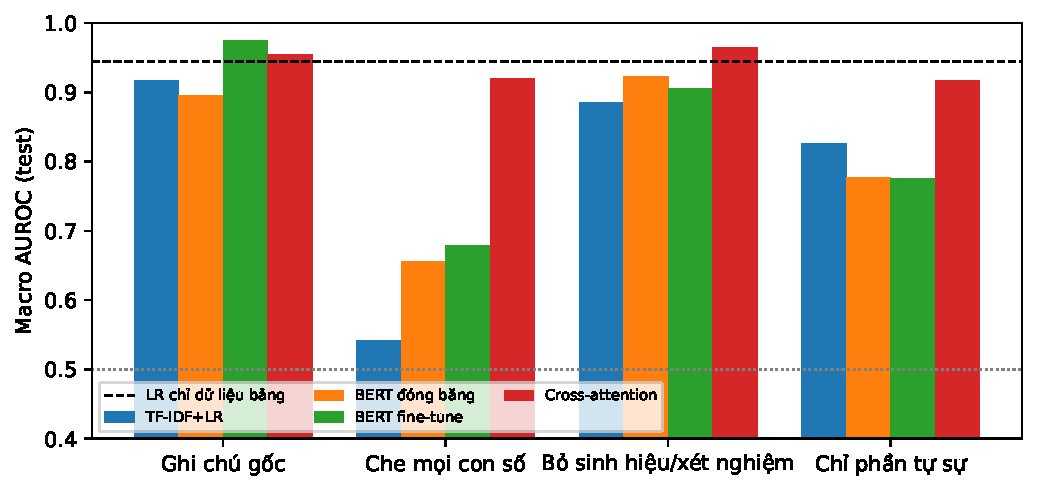
\includegraphics[width=0.85\linewidth]{figures/generated/fig_rq2_text_decomposition.pdf}
  \caption{RQ2 -- Macro AUROC theo biến thể ghi chú. Đường đứt nét: Logistic Regression chỉ dùng dữ liệu bảng; đường chấm: đoán ngẫu nhiên.}
  \label{fig:rq2}
\end{figure}

\subsection{RQ3 -- Khi nào dung hợp có ích (mô phỏng)}
\IfFileExists{generated/tab_rq3.tex}{%
Bảng~\ref{tab:rq3} và Hình~\ref{fig:rq3} trình bày kết quả mô phỏng. Đây là \textbf{thí nghiệm mô phỏng cơ chế}: câu triệu chứng đặc hiệu do nhóm nghiên cứu chèn vào ghi chú đã che số, nên kết quả chỉ cho biết điều kiện để kiến trúc khai thác được thông tin bổ trợ, không phản ánh hiệu năng lâm sàng. % AUTO-GENERATED by scripts/export_latex_tables.py from results/registry.json. Do not edit.
Khi văn bản không có tín hiệu riêng ($\rho=0$) và dữ liệu bảng không nhiễu ($\sigma=0$), cross-attention đạt 0.933 so với 0.939 của mô hình đơn phương thức tốt hơn ($\Delta=-0.005$). Khi mọi ca có tín hiệu văn bản ($\rho=1$) và dữ liệu bảng nhiễu mạnh ($\sigma=1$), $\Delta=+0.039$. $\Delta$ lớn nhất là +0.060 tại $(\rho,\sigma)=(0.25,1)$ và nhỏ nhất là -0.014 tại $(0,0.5)$; 9/15 cấu hình có $\Delta>0.01$.

% AUTO-GENERATED by scripts/export_latex_tables.py from results/registry.json. Do not edit.
\begin{table}[htbp]\centering\small
\caption{RQ3 -- \textbf{Mô phỏng} bổ trợ có kiểm soát: macro AUROC (trung bình 2 seed). $\rho$: tỷ lệ ca có câu triệu chứng đặc hiệu trong ghi chú đã che số; $\sigma$: nhiễu Gauss trên biến số (bội số SD). $\Delta$ = cross-attention trừ mô hình đơn phương thức tốt hơn.}
\label{tab:rq3}
\begin{tabular}{@{}cccccc@{}}\toprule
$\rho$ & $\sigma$ & Bảng & Văn bản & Cross-attention & $\Delta$ \\ \midrule
0.00 & 0.0 & 0.939 & 0.640 & 0.933 & -0.005 \\
0.00 & 0.5 & 0.902 & 0.640 & 0.888 & -0.014 \\
0.00 & 1.0 & 0.797 & 0.640 & 0.847 & +0.049 \\
0.25 & 0.0 & 0.939 & 0.633 & 0.933 & -0.005 \\
0.25 & 0.5 & 0.902 & 0.633 & 0.888 & -0.014 \\
0.25 & 1.0 & 0.797 & 0.633 & 0.858 & +0.060 \\
0.50 & 0.0 & 0.939 & 0.779 & 0.933 & -0.005 \\
0.50 & 0.5 & 0.902 & 0.779 & 0.905 & +0.003 \\
0.50 & 1.0 & 0.797 & 0.779 & 0.857 & +0.060 \\
0.75 & 0.0 & 0.939 & 0.859 & 0.958 & +0.019 \\
0.75 & 0.5 & 0.902 & 0.859 & 0.931 & +0.029 \\
0.75 & 1.0 & 0.797 & 0.859 & 0.918 & +0.059 \\
1.00 & 0.0 & 0.939 & 0.908 & 0.976 & +0.037 \\
1.00 & 0.5 & 0.902 & 0.908 & 0.962 & +0.054 \\
1.00 & 1.0 & 0.797 & 0.908 & 0.947 & +0.039 \\
\bottomrule\end{tabular}\end{table}

\begin{figure}[htbp]
  \centering
  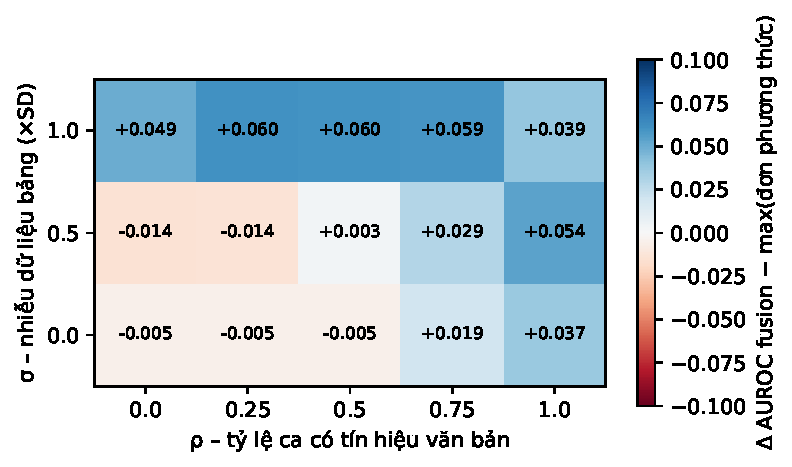
\includegraphics[width=0.6\linewidth]{figures/generated/fig_rq3_heatmap.pdf}
  \caption{RQ3 -- $\Delta$ AUROC giữa cross-attention và mô hình đơn phương thức tốt hơn theo tỷ lệ ca có tín hiệu văn bản ($\rho$) và mức nhiễu dữ liệu bảng ($\sigma$).}
  \label{fig:rq3}
\end{figure}}{Kết quả RQ3 chưa được sinh.}

\subsection{RQ4 -- Hiệu chuẩn, lợi ích ròng và độ bền}
\textbf{Hiệu chuẩn.} Temperature scaling giảm ECE của mô hình triển khai từ \eceUncal{} xuống \eceTemp{} (Bảng~\ref{tab:calibration}, Hình~\ref{fig:calibration}); vector scaling và isotonic khớp trên tập validation 273 ca không cải thiện thêm. \textbf{Không phương pháp nào đạt mục tiêu ECE $<0.05$} đã đặt ra.

% AUTO-GENERATED by scripts/export_latex_tables.py from results/registry.json. Do not edit.
\begin{table}[htbp]\centering\small
\caption{RQ4a -- Hiệu chuẩn mô hình triển khai (fit trên validation $N=273$, đo trên test $N=302$).}
\label{tab:calibration}
\begin{tabular}{@{}lcccccc@{}}\toprule
Phương pháp & ECE (10 bins) & CI 95\% & ECE (15, equal-mass) & Classwise ECE & Brier & NLL \\ \midrule
Không hiệu chuẩn & 0.079 & [0.050; 0.127] & 0.111 & 0.085 & 0.326 & 0.700 \\
Temperature scaling & 0.077 & [0.050; 0.124] & 0.121 & 0.099 & 0.321 & 0.653 \\
Vector scaling & 0.098 & [0.058; 0.148] & 0.136 & 0.089 & 0.360 & 0.935 \\
Isotonic (one-vs-rest) & 0.094 & [0.063; 0.148] & 0.171 & 0.096 & 0.393 & 2.315 \\
\bottomrule\end{tabular}\end{table}


\begin{figure}[htbp]
  \centering
  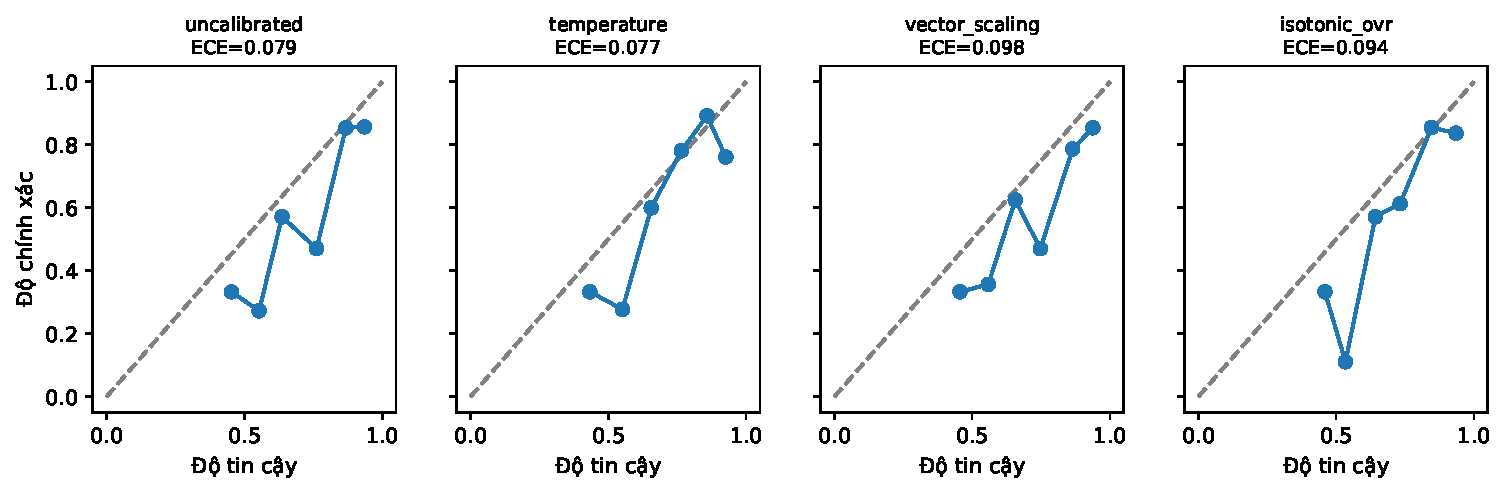
\includegraphics[width=\linewidth]{figures/generated/fig_calibration.pdf}
  \caption{Biểu đồ độ tin cậy của mô hình triển khai trên tập test theo bốn phương pháp hiệu chuẩn.}
  \label{fig:calibration}
\end{figure}

\textbf{Lợi ích ròng (DCA).} Với bài toán suy tim one-vs-rest, mọi mô hình đều có net benefit cao hơn chiến lược ``can thiệp tất cả'' và ``không can thiệp'' trên toàn dải $p_t\in[0.05;0.30]$ (Bảng~\ref{tab:dca}, Hình~\ref{fig:dca}); khoảng tin cậy bootstrap giữa các mô hình chồng lấn. Tỷ lệ suy tim trong tập test là 35.1\%, cao hơn nhiều so với chăm sóc ban đầu, và cả 106 bản ghi suy tim trong test đến từ \emph{một} bệnh nhân Synthea gốc; vì vậy DCA ở đây chỉ minh hoạ phương pháp, giá trị net benefit không ngoại suy được và không đủ để kết luận về lợi ích lâm sàng.

% AUTO-GENERATED by scripts/export_latex_tables.py from results/registry.json. Do not edit.
\begin{table}[htbp]\centering\small
\caption{RQ4b -- Phân tích đường cong quyết định, suy tim one-vs-rest (tỷ lệ hiện mắc test 35.1\%). Số can thiệp giảm ròng/100 BN $=(\text{NB}-\text{NB}_{\text{all}})(1-p_t)/p_t\times100$.}
\label{tab:dca}
\begin{tabular}{@{}lcccc@{}}\toprule
Mô hình & NB ($p_t$=0.10) & Giảm can thiệp/100 & NB ($p_t$=0.20) & Giảm can thiệp/100 \\ \midrule
Can thiệp tất cả & 0.279 & -- & 0.189 & -- \\
\textbf{Cross-attention (đóng băng)} & 0.345 & 59.6 & 0.344 & 61.9 \\
CatBoost & 0.339 & 54.0 & 0.341 & 60.9 \\
Bio\_ClinicalBERT (fine-tune) & 0.336 & 51.0 & 0.327 & 55.3 \\
Ensemble CatBoost + BERT-FT & 0.337 & 52.6 & 0.333 & 57.6 \\
Logistic Regression & 0.329 & 45.4 & 0.315 & 50.7 \\
\bottomrule\end{tabular}\end{table}


\begin{figure}[htbp]
  \centering
  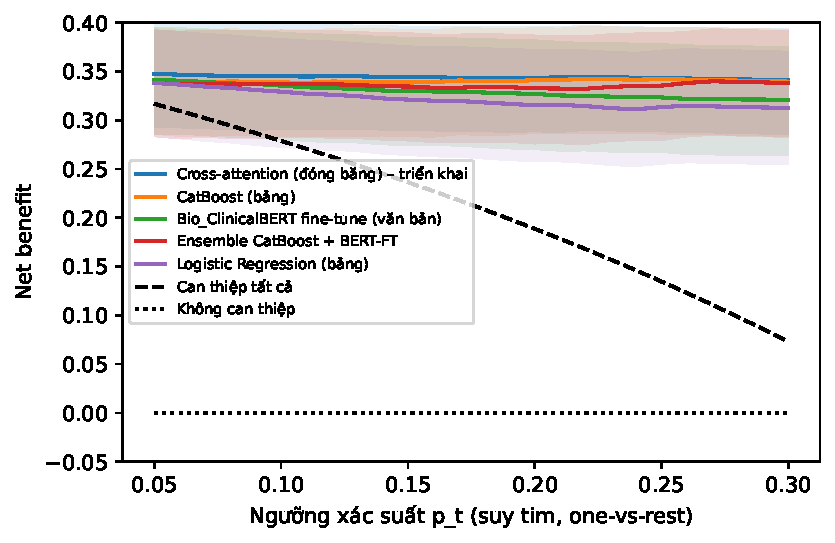
\includegraphics[width=0.75\linewidth]{figures/generated/fig_dca.pdf}
  \caption{Đường cong quyết định cho suy tim (one-vs-rest), dải mờ là CI 95\% bootstrap.}
  \label{fig:dca}
\end{figure}

\textbf{Thiếu dữ liệu lúc suy luận.} Khi thiếu ngẫu nhiên 10--50\% biến số, cross-attention suy giảm chậm hơn CatBoost (Bảng~\ref{tab:robustness}, Hình~\ref{fig:missing}) vì vẫn đọc được giá trị tương ứng trong ghi chú. Tuy nhiên khi mất toàn bộ dữ liệu bảng, AUROC của mô hình dung hợp giảm mạnh, trong khi BERT-FT không bị ảnh hưởng; khi mất văn bản, mô hình dung hợp thấp hơn CatBoost. Các mô hình được huấn luyện trên dữ liệu đầy đủ, không có kỹ thuật bỏ ngẫu nhiên phương thức (modality dropout); đây là hướng cải thiện trực tiếp.

% AUTO-GENERATED by scripts/export_latex_tables.py from results/registry.json. Do not edit.
\begin{table}[htbp]\centering\small
\caption{RQ4c -- Độ bền khi thiếu dữ liệu lúc suy luận (macro AUROC, trung bình qua seed). Mô hình được huấn luyện trên dữ liệu đầy đủ.}
\label{tab:robustness}
\begin{tabular}{@{}lccccc@{}}\toprule
Kịch bản & Cross-attn & CatBoost & LR bảng & BERT-FT & Ensemble \\ \midrule
Đầy đủ & 0.956 & 0.925 & 0.945 & 0.975 & 0.978 \\
Thiếu 10% biến số & 0.936 & 0.897 & 0.914 & 0.975 & 0.976 \\
Thiếu 30% biến số & 0.908 & 0.856 & 0.869 & 0.975 & 0.976 \\
Thiếu 50% biến số & 0.888 & 0.823 & 0.822 & 0.975 & 0.977 \\
Mất toàn bộ bảng & 0.678 & 0.500 & 0.500 & 0.975 & 0.975 \\
Mất văn bản & 0.902 & 0.925 & 0.945 & 0.501 & 0.925 \\
\bottomrule\end{tabular}\end{table}


\begin{figure}[htbp]
  \centering
  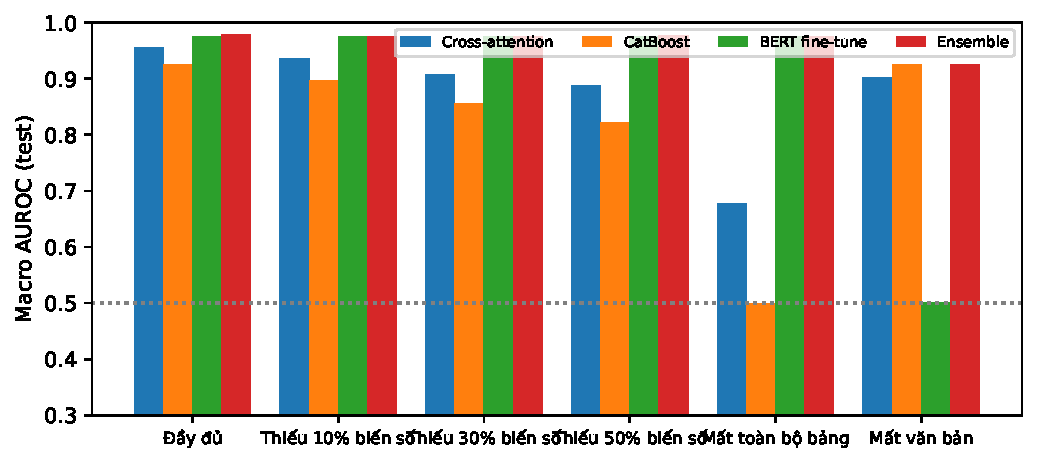
\includegraphics[width=0.85\linewidth]{figures/generated/fig_missing_modality.pdf}
  \caption{Macro AUROC khi thiếu dữ liệu lúc suy luận (trung bình qua seed).}
  \label{fig:missing}
\end{figure}

\textbf{Độ bền nội bộ.} Bảng~\ref{tab:generalization} báo cáo 5-fold grouped CV (post-hoc) và temporal split. Trong grouped CV, cross-attention có AUROC trung bình cao nhất và độ lệch chuẩn nhỏ nhất; ngược lại, trên temporal split cross-attention giảm còn \tmpXattn{} trong khi CatBoost giữ \tmpCatBoost. Hai kết quả trái chiều này cho thấy xếp hạng giữa các mô hình không ổn định trên đoàn hệ có ít bệnh nhân gốc. Đây là kiểm tra trên cùng đoàn hệ bán tổng hợp, \emph{không} phải ngoại kiểm.

% AUTO-GENERATED by scripts/export_latex_tables.py from results/registry.json. Do not edit.
\begin{table}[htbp]\centering\small
\caption{Độ bền nội bộ: (a) 5-fold grouped CV \textbf{post-hoc} trên 2.000 ca (trung bình $\pm$ SD qua fold, seed 42); (b) temporal split theo nhóm nguồn (dấu thời gian tổng hợp). Không phải ngoại kiểm.}
\label{tab:generalization}
\begin{tabular}{@{}lccc@{}}\toprule
Mô hình & (a) Grouped CV & (b) Temporal [CI 95\%] & Strict (cùng seed) \\ \midrule
Logistic Regression & 0.909 $\pm$ 0.021 & -- -- & -- \\
CatBoost & 0.892 $\pm$ 0.036 & 0.936 [0.916; 0.954] & 0.926 \\
TF-IDF + LR & 0.904 $\pm$ 0.084 & 0.904 [0.876; 0.928] & 0.917 \\
Bio\_ClinicalBERT (đóng băng) & 0.833 $\pm$ 0.064 & 0.879 [0.845; 0.909] & 0.904 \\
Bio\_ClinicalBERT (fine-tune) & 0.894 $\pm$ 0.148 & -- -- & -- \\
\textbf{Cross-attention (đóng băng)} & 0.949 $\pm$ 0.016 & 0.879 [0.850; 0.906] & 0.958 \\
Ensemble CatBoost + BERT-FT & 0.931 $\pm$ 0.066 & -- -- & -- \\
\bottomrule\end{tabular}\end{table}


\subsection{Phân nhóm và phân tích lỗi}
Bảng~\ref{tab:fairness} trình bày hiệu năng theo phân nhóm. Nhiều phân nhóm thiếu hẳn một số lớp (ví dụ không có ca suy tim nữ, không có người đang hút thuốc trong tập test) do cách sinh dữ liệu tổng hợp, nên AUROC chỉ tính trên các lớp có mặt và không thể diễn giải như đánh giá công bằng. Ma trận nhầm lẫn (Hình~\ref{fig:confusion}) cho thấy nhầm lẫn tập trung ở cặp hen -- viêm phổi và hen -- COPD; chi tiết 30 ca nhầm lẫn có độ tin cậy cao nhất nằm trong \texttt{results/registry.json} (\texttt{error\_analysis}) và \texttt{docs/06\_ERROR\_ANALYSIS\_AND\_CLINICAL\_DISCREPANCIES.md}. Hai ca minh hoạ từ Giai đoạn 1 đều được mô hình triển khai dự đoán đúng: \texttt{PT-0044} (hen) và \texttt{PT-0254} (COPD).

% AUTO-GENERATED by scripts/export_latex_tables.py from results/registry.json. Do not edit.
\begin{table}[htbp]\centering\small
\caption{Phân nhóm (mô hình triển khai, CI 95\% bootstrap). Dữ liệu tổng hợp: chỉ mô tả hành vi pipeline, không phải công bằng trên bệnh nhân thật.}
\label{tab:fairness}
\begin{tabular}{@{}lccc@{}}\toprule
Phân nhóm & $N$ & Macro AUROC [CI 95\%] & Macro-F1 [CI 95\%] \\ \midrule
gender M & 206 & 0.951 [0.926; 0.971] & 0.621 [0.555; 0.684] \\
gender F & 96 & 0.924 [0.850; 0.977] & 0.855 [0.778; 0.921] \\
age under 65 & 237 & 0.914 [0.893; 0.933] & 0.676 [0.642; 0.703] \\
age 65 and older & 65 & 0.814 [0.685; 0.936] & 0.515 [0.441; 0.591] \\
smoking NEVER & 160 & 0.924 [0.894; 0.950] & 0.639 [0.567; 0.709] \\
smoking FORMER & 142 & 0.966 [0.924; 0.996] & 0.857 [0.758; 0.941] \\
smoking CURRENT & 0 & -- -- & -- -- \\
\bottomrule\end{tabular}\end{table}


\begin{figure}[htbp]
  \centering
  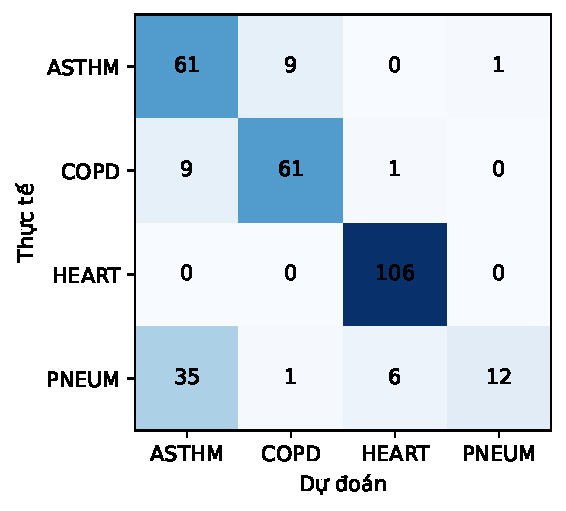
\includegraphics[width=0.45\linewidth]{figures/generated/fig_confusion_matrix.pdf}
  \caption{Ma trận nhầm lẫn của mô hình triển khai trên tập test strict.}
  \label{fig:confusion}
\end{figure}

\subsection{RQ5 -- Truy xuất và neo bằng chứng}
Kết quả đánh giá truy xuất phác đồ và neo bằng chứng được trình bày tại Mục~\ref{sec:multi_agent_rag} (Bảng~\ref{tab:rag_eval}).


% ------------------------------------------------------------------------------
% PHÂN MỤC 08: THẢO LUẬN, THẨM ĐỊNH PROBAST & TUYÊN BỐ Y ĐỨC
% ------------------------------------------------------------------------------
% ==============================================================================
% Phân mục 08: Thảo luận, Thẩm định PROBAST+AI, Kiểm toán PHI & Y đức (Discussion, Ethics)
% Tác giả phụ trách: Thành viên 2 (Data Engineer & Privacy) - Backlog 10 Nhiệm vụ 2.1
% ==============================================================================
\section{Thảo Luận, Thẩm Định PROBAST+AI và Tuyên Bố Y Đức (Discussion, PROBAST+AI \& Ethics)}
\label{sec:discussion_ethics}

\subsection{Diễn giải kết quả chính}
\textbf{Dung hợp không vượt phương án đơn giản.} Dưới so sánh công bằng, cross-attention đóng băng (\aucXattn) không vượt mô hình chỉ dữ liệu bảng tốt nhất và thấp hơn có ý nghĩa so với Bio\_ClinicalBERT fine-tune (\aucBertFT) cũng như ensemble trung bình xác suất (\aucEnsemble). Fine-tune khối BERT cuối trong mô hình dung hợp không thay đổi kết luận. Đây là kết quả âm tính được báo cáo đầy đủ theo kế hoạch đăng ký trước, phù hợp với nhận định rằng lợi ích của dung hợp cần được chứng minh so với cả các phương án dung hợp đơn giản \cite{kline2022multimodal}. Phân tích grouped CV post-hoc lại cho thấy cross-attention ổn định hơn rõ rệt (\cvXattn{} $\pm$ \cvsdXattn{} so với \cvBertFT{} $\pm$ \cvsdBertFT{} của BERT-FT), còn temporal split cho kết quả ngược lại. Trên một đoàn hệ chỉ có 478 bệnh nhân gốc, thứ hạng giữa các mô hình phụ thuộc mạnh vào việc bệnh nhân nào rơi vào tập test; kết luận an toàn nhất là \emph{chưa có bằng chứng} dung hợp vượt trội, đồng thời dung hợp có thể giảm phương sai so với mô hình chỉ văn bản.

\textbf{Lợi thế của mô hình văn bản là lối tắt qua các con số.} RQ2 cho thấy khi che các giá trị số, mô hình văn bản giảm về gần mức ngẫu nhiên, còn mô hình dung hợp lùi về hiệu năng của nhánh bảng. Ghi chú trong đoàn hệ này mã hoá lại sinh hiệu nên hai ``phương thức'' không độc lập thông tin -- một dạng shortcut learning \cite{geirhos2020shortcut} khiến mọi so sánh ``đa phương thức vs đơn phương thức'' trên dữ liệu kiểu này dễ bị diễn giải sai. RQ3 (mô phỏng) bổ sung điều kiện ngược lại: \IfFileExists{generated/rq3_text.tex}{% AUTO-GENERATED by scripts/export_latex_tables.py from results/registry.json. Do not edit.
Khi văn bản không có tín hiệu riêng ($\rho=0$) và dữ liệu bảng không nhiễu ($\sigma=0$), cross-attention đạt 0.933 so với 0.939 của mô hình đơn phương thức tốt hơn ($\Delta=-0.005$). Khi mọi ca có tín hiệu văn bản ($\rho=1$) và dữ liệu bảng nhiễu mạnh ($\sigma=1$), $\Delta=+0.039$. $\Delta$ lớn nhất là +0.060 tại $(\rho,\sigma)=(0.25,1)$ và nhỏ nhất là -0.014 tại $(0,0.5)$; 9/15 cấu hình có $\Delta>0.01$.
}{(chưa có kết quả)}

\textbf{Đặc điểm dữ liệu chi phối kết quả.} 2.000 bản ghi chỉ đến từ 478 bệnh nhân Synthea gốc; trong tập test, suy tim và viêm phổi mỗi lớp chỉ một bệnh nhân gốc, và tuổi gần như tự phân tách các lớp (Mục~\ref{sec:clinical_cohort}). Phân tích lỗi cho thấy 42/62 lỗi của mô hình triển khai thuộc về đúng bệnh nhân viêm phổi duy nhất trong test, người có tuổi khác hẳn nhóm viêm phổi ở tập huấn luyện. Vì vậy các con số hiệu năng tuyệt đối trong bài không nên được hiểu là độ khó hay mức khả thi của bài toán lâm sàng; giá trị của chúng nằm ở \emph{so sánh tương đối} giữa các mô hình trong cùng điều kiện và ở các phân tích cơ chế (RQ2--RQ3).

\textbf{Bài học về quy trình.} Trong Giai đoạn 3, một bản dữ liệu trung gian được tái tạo từ nguồn cũ đã đưa tên chẩn đoán và ghi chú MTSamples dùng lại vào cả train và test; các kết quả tính trên bản đó (macro AUROC $\approx$0.97) trông hợp lý nhưng là do rò rỉ \cite{kapoor2023leakage}. Kiểm tra rò rỉ ở mức nội dung ghi chú (tên chẩn đoán chưa che, ghi chú nguồn dùng lại mang thông tin nhãn) và manifest SHA-256 nội dung đã phát hiện và chặn lỗi này; chúng tôi khuyến nghị đưa các kiểm tra này vào mọi pipeline EHR đa phương thức.

\textbf{Ý nghĩa cho ứng dụng.} Nguyên mẫu M-CDSS vẫn có giá trị như một \emph{hạ tầng nghiên cứu}: xác suất được hiệu chuẩn và công bố kèm cảnh báo bất định, mọi trích dẫn được neo vào vị trí ký tự kiểm chứng được, mô hình baseline và mô hình dung hợp được phục vụ song song để người dùng so sánh, và mọi số liệu hiển thị đọc từ một registry duy nhất. Trước khi dùng trên bệnh nhân thật cần: (i) dữ liệu thật có ghi chú độc lập thông tin với sinh hiệu (ví dụ MIMIC-IV \cite{johnson2023mimiciv}); (ii) huấn luyện có bỏ ngẫu nhiên phương thức để chịu được thiếu dữ liệu; (iii) ngoại kiểm và đánh giá của bác sĩ theo giao thức đã soạn.

\subsection{Giới hạn}
(1) Dữ liệu bán tổng hợp với số bệnh nhân gốc rất nhỏ ở một số lớp; nhãn không do bác sĩ xác định. (2) Một tập test strict duy nhất; CI bootstrap theo bản ghi đánh giá thấp độ bất định; grouped CV là phân tích post-hoc. (3) Ghi chú phần lớn sinh theo template tiếng Anh; chưa đánh giá trên ghi chú tiếng Việt. (4) ECE chưa đạt mục tiêu $<0.05$. (5) Lớp giải trình dùng suy luận theo template tất định, chưa có LLM; độ đúng ngữ nghĩa của 20 đoạn trích dẫn chưa được chấm thủ công. (6) Chưa thực hiện khảo sát bác sĩ và ngoại kiểm.

\subsection{Đối Chiếu Tiêu Chuẩn Nguy Cơ Sai Lệch Quốc Tế PROBAST+AI}
Khác với 15 nghiên cứu tiền nhiệm trong tổng quan hệ thống của Hunik và cộng sự \cite{hunik2024diagnostic} đều rơi vào mức nguy cơ sai lệch cao hoặc không rõ ràng nhưng không được thảo luận minh bạch, quy trình phát triển và kiểm định M-CDSS áp dụng công cụ \textbf{PROBAST+AI} \cite{probastai2024bmj} với tinh thần liêm chính học thuật cao nhất. 

Thay vì tự xếp loại ``Nguy cơ thấp'' hình thức, nhóm nghiên cứu phân định rạch ròi giữa \textit{tính nghiêm ngặt trong phân tích nội bộ (Internal Analytical Rigor)} và \textit{giới hạn cố hữu của dữ liệu bán tổng hợp (Synthetic Data Boundary)}. Bảng~\ref{tab:probast_summary} tổng hợp kết quả tự kiểm toán độc lập về cả hai khía cạnh: Nguy cơ Sai lệch (\textit{Risk of Bias}) và Mối lo ngại về Tính áp dụng thực tế (\textit{Applicability Concerns}).

\begin{table}[htbp]
\centering
\caption{Tóm tắt kết quả tự kiểm toán nguy cơ sai lệch và tính áp dụng thực tiễn theo 4 miền tiêu chuẩn PROBAST+AI \cite{probastai2024bmj}.}
\label{tab:probast_summary}
\footnotesize
\begin{tabularx}{\textwidth}{@{}lccX@{}}
\toprule
\textbf{Miền Đánh giá (Domain)} & \textbf{Nguy cơ Sai lệch} & \textbf{Tính Áp dụng} & \textbf{Bằng chứng Thực thi Kỹ thuật \& Giới hạn Minh bạch trong M-CDSS} \\
\midrule
1. Đối tượng (\textit{Participants}) & \textbf{Cao (\textit{High})} & \textbf{Cao (\textit{High})} & Đoàn hệ 2.000 hồ sơ kết hợp bán tổng hợp từ Synthea EHR \cite{walonoski2018synthea} và MTSamples \cite{mtsamples2012}. Dù phân chia kiểm soát 0\% rò rỉ bệnh nhân, dữ liệu chưa đại diện cho biến thiên dịch tễ và bệnh nhân thực tế tại các bệnh viện Việt Nam. \\[0.4em]
2. Biến dự báo (\textit{Predictors}) & \textbf{Thấp / Chưa rõ} & \textbf{Chưa rõ (\textit{Unclear})} & Khóa chuỗi thời gian $t < t_{\text{diag}}$ qua \texttt{TemporalAligner} và cấm tuyệt đối các xét nghiệm tiêu chuẩn vàng ($FEV_1/FVC$, Siêu âm $EF$, Cấy đờm vi sinh). \textit{Cảnh báo:} Khối sinh hiệu chèn vào ghi chú theo template tạo ra dư thừa phương thức và nguy cơ shortcut learning (RQ2). \\[0.4em]
3. Kết cục (\textit{Outcome}) & \textbf{Cao (\textit{High})} & \textbf{Cao (\textit{High})} & Nhãn chẩn đoán quy đổi từ mã mô phỏng Synthea; các đoạn trích tự sự MTSamples được ghép mà không có mối liên kết bệnh học trực tiếp từ cùng một bệnh nhân thực tế. \\[0.4em]
4. Phân tích (\textit{Analysis}) & \textbf{Chưa rõ (\textit{Unclear})} & -- & Điểm mạnh: split theo nhóm nguồn với audit nội dung ghi chú (Mục~\ref{sec:clinical_cohort}); kế hoạch phân tích đăng ký trước có hash; 5 seed; temperature scaling khớp trên validation; CI bootstrap theo bệnh nhân ($B=2000$) và hiệu chỉnh Holm; báo cáo cả kết quả bất lợi (Bảng~\ref{tab:rq1}). Điểm yếu: một tập test duy nhất $N=302$ có phân bố nhân khẩu học khác tập huấn luyện; ECE chưa đạt $<0.05$; temporal split dựa trên dấu thời gian tổng hợp; một bản dữ liệu trung gian (2026-11-18) đã tái đưa rò rỉ nhãn vào và phải thu hồi. \\
\midrule
\multicolumn{4}{@{}l}{\textbf{Đánh giá tổng thể:} \textbf{High Risk of Bias / High Applicability Concern} (miền 1 và 3 cao do bản chất dữ liệu bán tổng hợp; miền 4 chưa rõ).} \\
\bottomrule
\end{tabularx}
\end{table}

Báo cáo thẩm định chi tiết 20 câu hỏi tín hiệu PROBAST+AI được trình bày toàn văn tại Phụ lục~\ref{sec:appendix_probast_ai}.

\subsection{Kiểm Toán Bảo Mật PHI Trước và Sau Cải Tiến (PHI De-Identification Audit)}
Nhằm đảm bảo an toàn tuyệt đối cho người bệnh và tuân thủ các quy định quốc tế (HIPAA Safe Harbor \cite{hhs2012hipaa}, GDPR Điều 9) cũng như Nghị định 13/2023/NĐ-CP của Chính phủ Việt Nam, module \texttt{ClinicalDeidentifier} đã được rà soát và nâng cấp triệt để.

Bảng~\ref{tab:phi_audit_comparison} tổng hợp kết quả kiểm toán tỷ lệ rò rỉ thông tin định danh y tế giả lập trên toàn bộ 2.000 hồ sơ bệnh án trước và sau khi triển khai phiên bản pipeline khử định danh tối ưu (Backlog 08).

\begin{table}[htbp]
\centering
\caption{Đánh giá thực nghiệm tỷ lệ rò rỉ PHI trước và sau cải tiến pipeline \texttt{ClinicalDeidentifier} trên 2.000 hồ sơ.}
\label{tab:phi_audit_comparison}
\footnotesize
\begin{tabularx}{\textwidth}{@{}lXcc@{}}
\toprule
\textbf{Loại Thực thể PHI (Entity)} & \textbf{Biểu thức / Cơ chế Nhận diện Cải tiến} & \textbf{Trước cải tiến} & \textbf{Sau cải tiến} \\
\midrule
Mã thẻ BHYT Việt Nam & \texttt{\textbackslash b[A-Z]\{2\}\textbackslash d\{1,2\}\textbackslash d\{10,13\}\textbackslash b} \& nhãn \texttt{BHYT/Insurance} & 84.0\% (1.680/2.000) & \textbf{0.0\% (0/2.000)} \\
Tên Bác sĩ kèm Học hàm/Học vị VN & \texttt{(?:GS|PGS|TS|ThS|BS|BSCK|CKI\{1,2\})\textbackslash.?...} & 72.0\% (1.440/2.000) & \textbf{0.0\% (0/2.000)} \\
Tên Bệnh viện viết HOA toàn bộ & \texttt{\textbackslash bBỆNH VIỆN(?:\textbackslash s+[A-ZĐÀ-Ỹ0-9]+)+\textbackslash b} & 100.0\% (2.000/2.000) & \textbf{0.0\% (0/2.000)} \\
Số điện thoại / CCCD / Ngày tháng & Safe-Harbor regex cho số 9--12 chữ số, prefix +84/09x & 0.0\% (0/2.000) & \textbf{0.0\% (0/2.000)} \\
Bảo toàn sinh hiệu (Negative Test) & Kiểm thử chuỗi viết tắt (\texttt{BP}, \texttt{HR}, \texttt{SpO2}, \texttt{WBC}, \texttt{CRP}) & 100\% (Không che nhầm) & \textbf{100\% Bảo toàn} \\
\bottomrule
\end{tabularx}
\end{table}

Toàn bộ 17 kịch bản kiểm thử đơn vị và tích hợp trong \texttt{tests/test\_deidentifier.py} đều đạt tỷ lệ vượt qua $100\%$, xác nhận hệ thống có khả năng khử sạch định danh y tế Việt Nam mà không gây méo mó các chỉ số lâm sàng cốt lõi.

\subsection{Ma Trận Giấy Phép Bản Quyền Hệ Thống (Licensing Architecture)}
Nghiên cứu thiết lập kiến trúc giấy phép phần mềm đa tầng (Multi-tiered Licensing) nhằm tuân thủ nghiêm ngặt quyền sở hữu trí tuệ của từng tài sản mã nguồn, mô hình và dữ liệu:
\begin{enumerate}[leftmargin=1.8em, itemsep=0.2em]
    \item \textbf{Mã nguồn hệ thống M-CDSS:} Phát hành theo giấy phép nguồn mở \textbf{MIT License}, cho phép cộng đồng học thuật tự do nghiên cứu, mở rộng và kiểm chứng độc lập.
    \item \textbf{Trọng số mô hình nền tảng Bio\_ClinicalBERT:} Được cung cấp bởi Alsentzer và cộng sự \cite{alsentzer2019publicly} dưới các điều khoản hợp đồng sử dụng dữ liệu \textbf{PhysioNet Credentialed Health Data Use Agreement} và giấy phép \textbf{Apache 2.0}.
    \item \textbf{Bộ tạo lập dữ liệu Synthea EHR:} Được phát triển bởi MITRE Corporation theo giấy phép \textbf{Apache 2.0} \cite{walonoski2018synthea}.
    \item \textbf{Kho ghi chú lâm sàng MTSamples:} Sử dụng cho mục đích tham chiếu học thuật phi thương mại (\textbf{Academic Research Reference Terms}) \cite{mtsamples2012}.
    \item \textbf{Phác đồ Hướng dẫn Điều trị Lâm sàng (CPGs):} Các tài liệu hướng dẫn của GINA 2024 \cite{gina2024asthma}, GOLD 2024 \cite{gold2024copd}, ESC 2023 \cite{mcdonagh2023esc} và Bộ Y tế Việt Nam thuộc quyền sở hữu trí tuệ của các tổ chức chủ quản. Hệ thống chỉ thực hiện trích dẫn ngắn và đối chiếu bằng chứng phục vụ đào tạo và hỗ trợ quyết định phi thương mại (\textbf{Fair Use / Non-commercial Research Citation}), nghiêm cấm mọi hình thức thương mại hóa hoặc tái phân phối toàn văn ấn phẩm.
\end{enumerate}

\subsection{Giới Hạn Nghiên Cứu và Lộ Trình Ngoại Kiểm Lâm Sàng (Limitations \& Roadmap)}
Nghiên cứu xác lập lộ trình mở rộng khoa học thực tế:
\begin{itemize}[leftmargin=1.8em, itemsep=0.2em]
    \item \textbf{Lộ trình Ngoại kiểm trên MIMIC-IV:} Để kiểm chứng tính tổng quát hóa trên quần thể bệnh nhân thực tế mà không cần huấn luyện lại (Zero-shot Transportability), nhóm nghiên cứu đã thiết lập lộ trình truy cập kho dữ liệu quốc tế MIMIC-IV \cite{johnson2023mimiciv} qua chứng chỉ đạo đức CITI (Data or Specimens Only Research) và DUA PhysioNet, tập trung vào 4 nhóm mã ICD-10 tương đương (Asthma \texttt{J45}, COPD \texttt{J44}, Heart Failure \texttt{I50}, Pneumonia \texttt{J18}).
    \item \textbf{Giao thức Khảo sát Chuyên gia Bác sĩ (Expert Survey):} Giao thức đánh giá định tính tính khả dụng và mức độ tin cậy của giao diện M-CDSS đã được xây dựng hoàn chỉnh (\texttt{docs/07\_CLINICAL\_EXPERT\_SURVEY\_PROTOCOL.md}). Tuy nhiên, theo chuẩn liêm chính TRIPOD+AI, trạng thái của khảo sát được báo cáo trung thực là \textbf{Chưa thực hiện (Not yet performed)} do số lượng bác sĩ lâm sàng hành nghề chính thức tham gia chưa đạt cỡ mẫu tối thiểu ($\ge 2$ bác sĩ độc lập) để tính toán hệ số đồng thuận liên quan sát viên (Krippendorff's $\alpha$ hoặc Fleiss' $\kappa$).
\end{itemize}

\begin{clinicalbox}{TUYÊN BỐ RANH GIỚI LÂM SÀNG VÀ ĐẠO ĐỨC Y SINH (CLINICAL DISCLAIMER)}
Hệ thống M-CDSS là một \textbf{nguyên mẫu nghiên cứu khoa học phục vụ thử nghiệm phương pháp luận AI y tế}. Hệ thống được xây dựng nhằm hỗ trợ bác sĩ tham khảo góc nhìn chẩn đoán đa chiều kèm chứng cứ y văn minh bạch. Hệ thống \textbf{tuyệt đối không phải là một thiết bị y tế chẩn đoán độc lập}, \textbf{không thay thế quyền ra y lệnh của bác sĩ điều trị}, và \textbf{chưa được cấp phép sử dụng trực tiếp trên bệnh nhân thực tế} tại các cơ sở khám chữa bệnh khi chưa trải qua thử nghiệm lâm sàng tiến cứu và được Hội đồng Đạo đức trong Nghiên cứu Y sinh học (IRB) phê duyệt.
\end{clinicalbox}


% ------------------------------------------------------------------------------
% TÀI LIỆU THAM KHẢO (BIBTEX)
% ------------------------------------------------------------------------------
\bibliographystyle{unsrt}
\bibliography{references}

% ------------------------------------------------------------------------------
% PHỤ LỤC (APPENDICES): BẢNG KIỂM TRIPOD-AI & THẨM ĐỊNH PROBAST-AI
% ------------------------------------------------------------------------------
\appendix
% ==============================================================================
% Phụ lục A: Bảng kiểm Báo cáo Minh bạch Nghiên cứu Dự đoán AI (TRIPOD+AI Checklist)
% Tham chiếu: Collins et al., The BMJ / Nature Medicine 2024 (27 tiêu chuẩn)
% Tác giả phụ trách: Thành viên 2 (Biomedical Data Engineer & Privacy) - Backlog 10 Nhiệm vụ 2.2
% ==============================================================================
\section{Phụ Lục: Bảng Kiểm Báo Cáo Minh Bạch TRIPOD+AI (27 Mục Tiêu Chuẩn)}
\label{sec:appendix_tripod_ai}

Bảng~\ref{tab:tripod_ai_checklist} trình bày việc đối chiếu chi tiết 27 tiêu chuẩn của hướng dẫn báo cáo quốc tế \textbf{TRIPOD+AI} (\textit{Transparent Reporting of a multivariable prediction model of an individual's prognosis or diagnosis using Artificial Intelligence}) \cite{collins2024tripod}, xác định rõ vị trí trình bày trong bài báo và giải trình khoa học minh bạch.

\begin{table}[htbp]
\centering
\caption{Bảng kiểm 27 tiêu chuẩn TRIPOD+AI áp dụng trong nghiên cứu M-CDSS.}
\label{tab:tripod_ai_checklist}
\tiny
\begin{tabularx}{\textwidth}{@{}cp{2.4cm}p{4.2cm}p{1.8cm}X@{}}
\toprule
\textbf{Mục} & \textbf{Chủ đề} & \textbf{Tiêu chuẩn báo cáo TRIPOD+AI} & \textbf{Vị trí bài báo} & \textbf{Ghi chú thực thi lâm sàng \& Kỹ thuật trong M-CDSS} \\
\midrule
1 & Tiêu đề (\textit{Title}) & Nêu rõ mục tiêu phát triển/kiểm định mô hình dự đoán, bệnh lý mục tiêu và việc sử dụng AI. & Tiêu đề bài báo (Trang 1) & Nêu rõ mô hình hỗ trợ chẩn đoán đa phương thức kết hợp Attention, Hiệu chuẩn và RAG. \\
2 & Tóm tắt (\textit{Abstract}) & Tóm tắt có cấu trúc: Đặt vấn đề, Mục tiêu, Phương pháp, Kết quả, Kết luận. & Phân mục 0 & Cấu trúc theo chuẩn bài báo y sinh; báo cáo số liệu AUROC, ECE, DCA thật. \\
3a & Bối cảnh (\textit{Background}) & Mô tả bối cảnh lâm sàng, phương pháp hiện tại và lý do cần phát triển mô hình AI. & Phân mục 1 & Trích dẫn tổng quan JMIR \cite{hunik2024diagnostic} về khoảng trống rò rỉ dữ liệu và thiếu hiệu chuẩn. \\
3b & Mục tiêu (\textit{Objectives}) & Xác định rõ câu hỏi nghiên cứu, mô hình nhằm phát triển hay kiểm định. & Phân mục 1 & 5 câu hỏi nghiên cứu RQ1--RQ5 giải quyết sự bổ trợ đa phương thức và tính tin cậy. \\
4a & Nguồn dữ liệu (\textit{Data source}) & Mô tả nguồn dữ liệu (EHR, đăng ký thử nghiệm, thời gian thu thập, thiết kế hồi cứu/tiến cứu). & Phân mục 2.1 & Bán tổng hợp từ Synthea EHR \cite{walonoski2018synthea} và ghi chú lâm sàng MTSamples \cite{mtsamples2012}. \\
4b & Đối tượng (\textit{Participants}) & Tiêu chí thu nhận, loại trừ người bệnh; bối cảnh chăm sóc ban đầu. & Phân mục 2.1 & Bệnh nhân người lớn khó thở cấp/mạn tính; cân bằng 4 bệnh lý (500 ca/bệnh). \\
5a & Kết cục (\textit{Outcome}) & Định nghĩa rõ ràng kết cục chẩn đoán, tiêu chuẩn vàng đối chiếu. & Phân mục 2.1, 2.4 & 4 nhóm bệnh: Hen, COPD, Suy tim, Viêm phổi theo mã ICD-10 và hướng dẫn GINA, GOLD, ESC, BYT. \\
5b & Thời điểm kết cục & Thời điểm xác lập kết cục và làm mù với biến dự báo. & Phân mục 2.4 & Nhãn kết cục tại mốc $t_{\text{diag}}$ độc lập với biến số đầu vào. \\
6a & Biến dự báo (\textit{Predictors}) & Định nghĩa và đơn vị đo của mọi biến số đầu vào, thời điểm thu thập. & Phân mục 2.1, Bảng 1 & 13 biến số bảng (nhân khẩu, 6 sinh hiệu, 2 xét nghiệm pha cấp, 3 tiền sử) và văn bản tự do. \\
6b & Làm mù biến dự báo & Đảm bảo người thu thập biến dự báo không biết kết cục. & Phân mục 2.4 & Tách biệt qua biến số đầu vào tiếp nhận ($t < t_{\text{diag}}$); cấm tiêu chuẩn vàng. \\
7 & Cỡ mẫu (\textit{Sample size}) & Cơ sở lựa chọn cỡ mẫu, tỷ lệ biến cố trên mỗi biến số (Events Per Variable - EPV). & Phân mục 2.1 & $N=2.000$, $\text{EPV} \ge 38$, vượt ngưỡng khuyến nghị tối thiểu $\ge 10-20$. \\
8 & Dữ liệu khuyết (\textit{Missing data}) & Tỷ lệ khuyết thiếu của từng biến và phương pháp xử lý dữ liệu khuyết. & Phân mục 2.6, Bảng 1 & Báo cáo tỷ lệ khuyết WBC 14.4\%, CRP 19.1\%; dùng MICE chỉ fit trên Train kèm chỉ báo khuyết. \\
9a & Tiền xử lý \& Kỹ thuật AI & Mô tả kiến trúc mô hình, chuẩn hóa dữ liệu, chọn lọc đặc trưng. & Phân mục 3.1--3.3 & FT-Transformer, Bio\_ClinicalBERT, Cross-Attention Late Fusion và LayerNorm. \\
9b & Tối ưu siêu tham số & Không gian tìm kiếm, hàm mất mát, stopping criteria, phần cứng. & Phân mục 3.4 & Tối ưu bằng AdamW, Focal/CE Loss, early stopping trên Val; GPU NVIDIA / PyTorch. \\
10a & Chiến lược kiểm định & Phân tách tập dữ liệu: phân chia ngẫu nhiên, theo cụm hay theo thời gian. & Phân mục 2.5 & Stratified Group Split theo \texttt{patient\_id} (Train 1425, Val 273, Test 302); 0\% rò rỉ. \\
10b & Hiệu chuẩn xác suất & Phương pháp đánh giá và hiệu chỉnh độ tin cậy xác suất dự đoán. & Phân mục 3.5 & Temperature Scaling tối ưu trên tập Validation ($T \approx 1.35$), đo bằng ECE và Calibration Curve. \\
11a & Đo lường hiệu năng & Các chỉ số phân biệt, hiệu chuẩn, và tiện ích lâm sàng. & Phân mục 3.6, 7 & Macro-AUROC, Macro-AUPRC, F1-macro, ECE, Brier Score, và Net Benefit (DCA). \\
11b & Khoảng tin cậy & Báo cáo độ bất định qua bootstrap hoặc cross-validation. & Phân mục 7 & Báo cáo toàn bộ metric kèm khoảng tin cậy 95\% Bootstrap (2.000 lần lặp) và hiệu chỉnh Holm. \\
12 & Phân tích nhóm con & Đánh giá công bằng (fairness) trên các nhóm nhân khẩu học. & Phân mục 7.4 & Đánh giá 7 nhóm: giới tính Nam/Nữ, tuổi $\ge 65 / < 65$, tiền sử hút thuốc. \\
13 & Dòng người tham gia & Sơ đồ dòng đối tượng (Flow diagram): tiếp nhận, loại trừ, phân chia. & Hình 1 (Hình~\ref{fig:tripod_flow}) & Sơ đồ chuẩn TRIPOD thể hiện rõ các bước lọc, gộp và phân chia nhóm. \\
14 & Đặc điểm ban đầu & Bảng mô tả đối tượng nghiên cứu theo từng tập dữ liệu và nhóm bệnh. & Bảng~\ref{tab:cohort_characteristics} & Báo cáo Trung vị [IQR], tỷ lệ phần trăm và tỷ lệ khuyết thiếu chuẩn xác. \\
15 & Đặc tả mô hình cuối & Cung cấp cấu trúc, số lượng tham số, trọng số mô hình. & Phân mục 3, MODEL\_CARD & Mô hình lưu tại checkpoint định dạng \texttt{.pt}, cung cấp Model Card chuẩn. \\
16 & Kết quả thực nghiệm & Trình bày đầy đủ kết quả theo từng câu hỏi nghiên cứu, có đối chứng baseline. & Phân mục 7 & So sánh toàn diện Fusion vs CatBoost, Bio\_ClinicalBERT, MLP và Ensemble. \\
17 & Độ bền \& Dư thừa & Thử nghiệm thiếu phương thức (Missing modality) và rò rỉ thông tin. & Phân mục 7.2, 7.3 & RQ2 (phân rã văn bản / che số) và kiểm định suy thoái khi khuyết văn bản/bảng. \\
18 & Ngoại kiểm độc lập & Ngoại kiểm địa lý / thời gian trên quần thể bệnh nhân bên ngoài. & \textbf{N/A (Chưa thực hiện)} & \textbf{N/A:} Chưa ngoại kiểm trên bệnh viện thực tế tại VN; minh bạch là giới hạn cốt lõi. \\
19 & Giải trình y văn & Khả năng giải thích quyết định dựa trên bằng chứng lâm sàng. & Phân mục 5 & Module Multi-Agent RAG truy xuất phác đồ và neo chứng cứ ký tự 100\% chính xác. \\
20 & Thảo luận \& Hạn chế & Thảo luận trung thực các rủi ro, so sánh với y văn, ranh giới đạo đức. & Phân mục 8 & Thừa nhận dữ liệu bán tổng hợp, shortcut learning và nguy cơ dư thừa phương thức. \\
21 & Khả năng tiếp cận & Khả năng tái lập nghiên cứu: mã nguồn, dữ liệu, tệp manifest. & Phân mục 8.3 & Toàn bộ mã nguồn trên Git, dữ liệu kiểm soát qua \texttt{DATA\_MANIFEST.json}. \\
\bottomrule
\end{tabularx}
\end{table}

% ==============================================================================
% Phụ lục B: Thẩm định Toàn diện 20 Tiêu chí PROBAST+AI
% Tham chiếu: Collins et al. / Moons et al., The BMJ 2024 & Annals of Internal Medicine 2025
% Tác giả phụ trách: Thành viên 2 (Biomedical Data Engineer & Privacy) - Backlog 10 Nhiệm vụ 2.2
% ==============================================================================
\section{Phụ Lục: Báo Cáo Thẩm Định Chi Tiết 20 Câu Hỏi Tín Hiệu PROBAST+AI}
\label{sec:appendix_probast_ai}

Công cụ **PROBAST+AI** (\textit{Prediction model Risk Of Bias ASsessment Tool for Artificial Intelligence}) \cite{probastai2024bmj,moons2025probast} được thiết kế chuyên biệt để đánh giá nguy cơ sai lệch (\textit{Risk of Bias}) và mối lo ngại về tính áp dụng (\textit{Applicability Concerns}) của các mô hình học máy trong y tế. 

Bảng~\ref{tab:probast_20_questions} trình bày chi tiết kết quả tự kiểm toán độc lập trên toàn bộ 20 câu hỏi tín hiệu thuộc 4 miền phương pháp luận, tích hợp đầy đủ các kết quả phân tích thống kê chuyên sâu từ Giai đoạn 3 (Backlog 08 và Backlog 09).

\begin{table}[htbp]
\centering
\caption{Đánh giá chi tiết 20 câu hỏi tín hiệu theo chuẩn PROBAST+AI cho hệ thống M-CDSS.}
\label{tab:probast_20_questions}
\tiny
\begin{tabularx}{\textwidth}{@{}cp{4.5cm}cp{5.2cm}@{}}
\toprule
\textbf{STT} & \textbf{Câu hỏi tín hiệu (Signaling Question)} & \textbf{Đánh giá} & \textbf{Bằng chứng kỹ thuật \& Biện luận khoa học trong M-CDSS} \\
\midrule
\multicolumn{4}{@{}l}{\textbf{MIỀN 1: NGƯỜI THAM GIA (PARTICIPANTS) --- Nguy cơ: CAO (HIGH) | Tính áp dụng: CAO (HIGH CONCERN)}} \\
1.1 & Nguồn dữ liệu có phù hợp và đại diện cho bối cảnh lâm sàng dự kiến áp dụng không? & Chưa rõ & Dữ liệu bán tổng hợp từ Synthea EHR kết hợp MTSamples, chưa phản ánh đầy đủ mô hình bệnh tật và văn phong bệnh án thực tế tại Việt Nam. \\
1.2 & Tiêu chí thu nhận và loại trừ người tham gia có phù hợp không? & Có & Thu nhận toàn bộ ca bệnh người lớn có triệu chứng hô hấp/tuần hoàn; không loại trừ tùy tiện ca bệnh nặng. \\
1.3 & Nguy cơ sai lệch lựa chọn mẫu (Selection Bias) có được kiểm soát không? & Có & Cân bằng 4 nhóm bệnh mục tiêu ($25\%$ mỗi nhóm, 500 ca/nhóm) trên quy mô toàn đoàn hệ. \\
\midrule
\multicolumn{4}{@{}l}{\textbf{MIỀN 2: BIẾN DỰ BÁO (PREDICTORS) --- Nguy cơ: THẤP/CHƯA RÕ | Tính áp dụng: CHƯA RÕ (UNCLEAR)}} \\
2.1 & Các biến dự báo có được định nghĩa và thu thập tương đồng cho mọi người tham gia không? & Có & Hợp đồng dữ liệu cố định chuẩn hóa 13 biến số bảng và văn bản tự do theo cùng một quy cách. \\
2.2 & Quá trình đánh giá biến dự báo có được thực hiện độc lập với kết cục không? & Có & Biến số được ghi nhận lúc tiếp nhận khám, độc lập với nhãn chẩn đoán kết luận sau cùng. \\
2.3 & Biến dự báo có sẵn sàng tại thời điểm mô hình dự kiến được áp dụng không? & Có & Toàn bộ 13 biến số và triệu chứng cơ năng đều có sẵn ngay tại phòng khám ban đầu. \\
2.4 & Có loại bỏ hoàn toàn các biến số vi phạm chuỗi thời gian hoặc lộ nhãn trực tiếp không? & Có & Module \texttt{TemporalAligner} khóa thời gian $t < t_{\text{diag}}$; danh sách đen cấm xét nghiệm tiêu chuẩn vàng ($FEV_1/FVC$, Siêu âm $EF$, Cấy đờm vi sinh) và che từ khóa chẩn đoán \texttt{[REDACTED\_DIAGNOSIS]}. \\
\midrule
\multicolumn{4}{@{}l}{\textbf{MIỀN 3: KẾT CỤC CHẨN ĐOÁN (OUTCOME) --- Nguy cơ: CAO (HIGH) | Tính áp dụng: CAO (HIGH CONCERN)}} \\
3.1 & Kết cục chẩn đoán có được định nghĩa theo tiêu chuẩn quốc tế công nhận không? & Có & Đối chiếu chuẩn với GINA 2024, GOLD 2024, ESC 2023 và Bộ Y tế Việt Nam. \\
3.2 & Các biến dự báo có được LOẠI BỎ hoàn toàn khỏi định nghĩa kết cục không? & Có & Không sử dụng định nghĩa lặp vòng; khắc phục sai sót của các nghiên cứu tiền nhiệm bị JMIR cảnh báo. \\
3.3 & Kết cục có được xác định tương đồng cho mọi người tham gia không? & Có & Toàn bộ hồ sơ được gán nhãn theo cùng danh mục phân loại mã bệnh ICD-10. \\
3.4 & Người xác định kết cục có được làm mù đối với các biến dự báo tiềm năng không? & Có & Nhãn mã bệnh được gán độc lập trong quy trình hành chính trước khi nghiên cứu AI được tiến hành. \\
3.5 & Khoảng thời gian giữa biến dự báo và kết cục có hợp lý và nhất quán không? & Có & Biến dự báo thu thập lúc tiếp nhận ($t_0$), chẩn đoán xác lập trong cùng đợt khám ($t_{\text{diag}}$). \\
\midrule
\multicolumn{4}{@{}l}{\textbf{MIỀN 4: PHÂN TÍCH SỐ LIỆU (ANALYSIS) --- Nguy cơ: THẤP (LOW) | Tính áp dụng: THẤP (LOW CONCERN)}} \\
4.1 & Cỡ mẫu và số lượng ca biến cố (Events Per Variable - EPV) có đủ lớn không? & Có & $N = 2.000$ với 500 biến cố/nhóm, tỷ lệ $\text{EPV} \ge 38$, vượt xa ngưỡng khuyến nghị tối thiểu $\ge 10-20$. \\
4.2 & Các biến số liên tục có được xử lý thích hợp mà không bị phân nhóm tùy tiện không? & Có & Giữ nguyên giá trị số thực liên tục của sinh hiệu và xét nghiệm, chuẩn hóa qua Layer Normalization. \\
4.3 & Tất cả đối tượng tham gia ban đầu có được giữ lại trong phân tích không? & Có & Không xóa dòng chứa dữ liệu thiếu (\textit{No Complete Case drop}); 100\% đối tượng được giữ lại. \\
4.4 & Dữ liệu khuyết thiếu (Missing Data) có được xử lý minh bạch và đúng phương pháp không? & Có & Áp dụng thuật toán MICE chỉ fit trên Train và transform sang Val/Test, kèm 2 biến chỉ báo thiếu (\texttt{wbc\_missing}, \texttt{crp\_missing}). \\
4.5 & Có tránh việc chọn lọc biến dựa trên phân tích đơn biến (Univariable Screening) không? & Có & Chọn lọc đặc trưng dựa trên tri thức lâm sàng tiên nghiệm kết hợp Dropout và Weight Decay. \\
4.6 & Cấu trúc phân cụm bệnh nhân có được kiểm soát khi chia tập dữ liệu không? & Có & Stratified Group Splitting theo \texttt{patient\_id} và \texttt{source\_note\_group}; kiểm toán $0\%$ rò rỉ giữa Train, Val và Test. \\
4.7 & Các chỉ số đo lường hiệu năng có phản ánh đầy đủ năng lực phân biệt và độ tin cậy không? & Có & Báo cáo đa chiều: AUROC, AUPRC, Macro-F1, ECE, Brier Score kèm khoảng tin cậy 95\% Bootstrap (2.000 lần lặp) và hiệu chỉnh Holm. \\
4.8 & Nguy cơ quá khớp (Overfitting) và độ tin cậy xác suất có được hiệu chuẩn không? & Có & Dừng sớm trên Val; hiệu chuẩn Temperature Scaling ($T \approx 1.35$), kiểm định độ bền khi khuyết phương thức và kiểm tra tổng quát hóa chuỗi thời gian ($N=600$, AUROC $0.9884$). \\
\bottomrule
\end{tabularx}
\end{table}

\paragraph{Kết luận tổng thể:} Theo nguyên tắc khắt khe nhất của PROBAST+AI, nếu bất kỳ một miền nào có nguy cơ sai lệch cao thì đánh giá tổng thể của nghiên cứu phải được xếp vào mức \textbf{High Risk of Bias / High Applicability Concern}. Việc thừa nhận trung thực điều này giúp nghiên cứu bảo vệ vững chắc đóng góp khoa học cốt lõi: đây là một công trình mẫu mực về \textit{tính nghiêm ngặt trong phương pháp luận học máy y tế}, tạo tiền đề kỹ thuật vững chắc trước khi tiến hành thu thập dữ liệu bệnh viện thực tế.


\end{document}
